\chapter{実験}
\label{chap:result}
\fancyhf{}
\rhead{\thepage}
\lhead{第\ref{chap:result}章 実験}
\cfoot{\thepage}


本章では,実験について述べる.

提案手法によって学習・抽出した知識分類が,
実際にどの程度の予測性能を持ち,
またその性能が知識分類のどのような性質に起因するのかを,
3つの実験によって分析・検証する.
以下では,まず,それぞれの実験について実験設定を述べ,
その後,実験結果について述べる.


\section{実験設定}

本研究の実験は,大きく以下の3つに分けられる.
\begin{enumerate}
	\item 知識分類の学習と抽出
	\item 知識分類の予測性能の検証
	\item 知識分類の性質の比較
\end{enumerate}
以下では,順に,実験設定について述べる.


\subsection{知識分類の学習と抽出}
\label{sec:section}
生徒の問題回答ログに対し,図\ref{fig:model}に表される知識分類学習モデルを適用し,
問題空間を知識タグ空間に最適に変換する写像行列を学習し,
離散化してタグとして抽出する.

知識タグ空間の次元数は,既存の知識分類の次元数と統一し,
「ASSISTments 2009-2010」では55,
「Bridge to Algebra 2006-2007」では115とした.
実際のモデルにおいては,正答ベクトルと誤答ベクトルを分けてユニットを作るため,
それぞれ2倍のユニット数で表現されている.

RNNの部分にはGRNNを用いる.
ハイパーパラメータについては,
学習率の初期値を$150$,
モーメントを$0.98$,
1エポックごとに,
減衰率$0.99$として学習率を最小学習率$10$まで減衰させる.
また,勾配のノルムの最大値を$0.00001$として\cite{pascanu2013difficulty}に従い勾配に制約を設けた.
dropoutは${\bf u}_t$から${\bf h}_t$の方向にdropout率$0.2$,${\bf h}_t$から${\bf y}_t$の方向にdropout率$0.5$で適用した.
隠れ層のユニット数は$400$として,
各重み行列の初期化は\cite{glorot2010understanding}に従った.
時系列方向の誤差逆伝搬は最長で$200$まで伝搬するように制約を設けた.

これらのハイパーパラメータは実験的に高い予測性能を発揮したため設定しており,
網羅的に探索したわけではない.
通常,深層学習の手法はハイパーパラメータの数が非常に大きく,また,
計算コストが大きいため大規模な探索は行えない.
Grid SearchやRandom Search\cite{bergstra2012random}といった探索手法が提案されているが,
専門家が手で調整した方が優れていることが報告されている\cite{larochelle2007empirical, bergstra2012random}.

最適化手法は,
式\ref{eq:prediction_entropy}で表される問題回答予測に関する誤差関数$L_p$と,
式\ref{eq:autoencoder_loss}で表される問題空間と知識タグ空間の再構成誤差$L_r$,
式\ref{eq:sparse}で表されるスパース正則化項$L_s$
の和である
$L$(式\ref{eq:total_loss})を目的関数として最小化するものである.
学習時は\cite{piech2015deep}と同様にミニバッチごとに確率的勾配降下法で目的関数を最小化する.
評価指標はAUCスコアを採用する.

2つのデータセットいずれにおいても,
訓練:検証:テスト = 8:1:1となるようにユーザを分け,
訓練ユーザのデータでモデルを構築し,
検証ユーザのデータでハイパーパラメータを調整し, 
検証ユーザのデータで精度が最も高かったモデルから写像行列を抽出した.

%一般的な機械学習では,モデルの汎化性能を高めるために訓練データと検証データを分けるが,
%2つのデータセットいずれにおいても,全ユーザの問題回答ログを訓練データとして,モデルを学習させた.
%これは,分類を作成する時点において既知のデータから帰納的に最適な知識分類を作成するという本研究のテーマと,
%未知のデータが追加される都度モデルを学習させ,知識分類を更新することが容易であるオンライン教育サービスのプラットフォームの環境を考慮し,
%最適な問題設定としたものである.
%この設計と知識分類の汎用性に関しては第6章で詳述する.

得られた写像行列を以下の条件に基づいて離散化し,タグとして抽出する.
%DKTにおいて最も高い精度を発揮したものをその手法による精度の上界として採用し,
「ASSISTments 2009-2010」では$Y = 0.85$,「Bridge to Algebra 2006-2007」では$Y = 0.??$とした.
\begin{enumerate}
\item 各問題の写像ベクトルにおいて,最も値が大きいタグを1とする.
\item 写像行列全体において,値が閾値$Y$以上のタグを1とする.
\item 写像行列全体において,1でない要素を0にする.
\end{enumerate}

実装には
Theano\cite{bergstra+al:2010-scipy,Bastien-Theano-2012}を用いた.
Theanoは多次元行列を含む数学的表現の定義や計算,最適化を効率的に行えるPythonのライブラリで,
深層学習の研究ではよく利用される.


\subsection{知識分類の予測性能の検証}

\ref{sec:section}で抽出した知識分類をDeep Knowledge Tracing(DKT)に用いて知識獲得予測を行い,
既存の知識分類を用いた場合との精度の比較を行う.
また,本手法で抽出される知識分類と既存の知識分類の差分を明確にするため,
以下の方法で作成された知識分類を用いた場合とも比較を行う.
\begin{itemize}
\item 回答正誤予測の文脈を考慮せず,一般的な事前学習のAutoencoderによって作成された知識分類\label{c1}
\item 回答正誤予測の文脈を考慮するが,学習時の損失関数に再構成誤差やスパース正則化項を導入せずに作成された知識分類\label{c2}
\end{itemize}

RNNの部分にはGRNNを用いる.
ハイパーパラメータについては,
学習率の初期値を$100$,
モーメントを$0.98$,
1エポックごとに,
減衰率$0.9$として学習率を最小学習率$10$まで減衰させる.
また,勾配のノルムの最大値を$0.00001$として\cite{pascanu2013difficulty}に従い勾配に制約を設けた.
dropoutは\cite{piech2015deep}と同様に${\bf y}_t$の方向にのみかけ,
dropout率は$0.5$とした.
隠れ層のユニット数は$400$として,
各重み行列の初期化は\cite{glorot2010understanding}に従った.
時系列方向の誤差逆伝搬は最長で$200$まで伝搬するように制約を設けた.

最適化手法は,
一般的なDKTと同じく,
式\ref{eq:prediction_entropy}で表される回答正誤予測に関する誤差関数$L_p$
を目的関数として最小化するものである.
学習時は\cite{piech2015deep}と同様にミニバッチごとに確率的勾配降下法で目的関数を最小化する.
評価指標はAUCスコアを採用する.

2つのデータセットいずれにおいても,
\ref{sec:section}でのデータ分割に基づき,
訓練ユーザのデータでモデルを構築し,
検証ユーザのデータでハイパーパラメータを調整し, 
検証ユーザのデータで精度が最も高かったモデルを
テストユーザのデータに適用し当該モデルの最終的な精度とした.

実装にはTheanoを用いた.


\subsection{知識分類の性質の比較}

\ref{sec:section}で抽出された知識分類を既存の知識分類と比較分析することで,その性質を検証する.

まず,既存の知識分類(以下,既存タグ)と抽出された知識分類(以下,抽出タグ)それぞれにおいて,各タグが回答ログに出現する回数の分布に着目し,
知識獲得予測の精度を向上させる要因を,データ構造の側面から定量的に分析する.

次に,抽出タグと既存タグの関係性を可視化し,その構造や内容について比較を行う.
図\ref{fig:networkflow}の手順に従って,
既存タグネットワークとタグ関係行列を算出し,
こタグ関係行列を元に抽出タグのノードを既存タグネットワークに追加することで,両タグの関係性を表す「タグ関係ネットワーク」を作成する.

まず,既存タグをノードとする知識間影響ネットワーク(以下,既存タグネットワーク)を,既存のDKTで用いられた手法に基づいて作成し.
次に,抽出タグと既存タグの共起行列に対してTF-IDF法を適用して各抽出タグの特徴を強調し,抽出タグと既存タグの関係性を表す行列(以下,タグ関係行列)を作成し,
この行列を元に抽出タグのノードを既存タグネットワークに追加することで,両タグの関係性を表す「タグ関係ネットワーク」を作成する.
ここで,既存タグネットワークでは,
ノードのサイズは,各既存タグの回答ログにおける出現回数に比例して設定し,
ノードの色は,回答ログにおける平均回答順序が早いものほど青く,遅いものほど赤く色を設定し,
各既存タグへの影響度が大きい上位3つの既存タグからエッジを引く.
また,タグ関係ネットワークにおいて追加される抽出タグは緑色のノードで表現し,
各抽出タグにとって関係性の強い上位3つの既存タグに対して緑色のエッジを引く.




\section{実験結果}
実験結果について述べる.
まず,各手法によって作成された知識分類についての知識獲得予測における予測性能を比較し,
いずれのデータセットにおいても,
提案手法によって抽出された知識分類が最も良い精度を記録したことを定量的に確認する.

さらに,抽出された知識分類を,既存の知識分類と比較することにより,その性質を定量的・定性的に分析する.



\subsection{知識分類の予測性能の比較}

\begin{table}[!htb]
%\begin{table}[t]
\caption{各知識分類の知識獲得予測における予測性能}
\label{tab:result1}
\begin{center}
\scalebox{0.9}{
\centerline{
{
%\begin{tabular}{c|ccccc}\hline
%\multirow{3}{*}{データセット}	&	\multicolumn{5}{c}{AUC}\\\cline{2-6}
% 							&	\multirow{2}{*}{既存タグ(marginal)} 	& \multirow{2}{*}{事前学習タグ} 	&	& \multicolumn{2}{c}{提案手法タグ}\\\cline{5-6}
%							&										& 								&	& Embedding 	& AutoEncoder \\\hline 			 
%ASSISTments 2009-2010  		&				0.72 (0.61) 			& 			0.67 				& 	& 0.69 			& {\bf 0.74} \\
%Bridge to Algebra 2006-2007 &				0.81 (0.72) 			& 			0.79 				& 	& 0.81 			& {\bf 0.82} \\
%\hline
%\end{tabular}
\begin{tabular}{c|cccccc}\hline
\multirow{3}{*}{データセット}	&	\multicolumn{6}{c}{AUC}\\\cline{2-7}
 							&	\multirow{2}{*}{既存タグ(marginal)} 	& \multirow{2}{*}{事前学習タグ} 	&	& \multicolumn{3}{c}{提案手法タグ}\\\cline{5-7}
							&										& 								&	& 	$L_p$	& $L_p + L_r$	& $L_p + L_r + L_s$ \\\hline 			 
ASSISTments 2009-2010  		&				0.72 (0.60) 			& 			0. 					& 	& 	 		&  				&		{\bf 0.73}	\\
Bridge to Algebra 2006-2007 &				0.78 (0.70) 			& 			0. 					& 	& 	 		& 			 	&		{\bf 0.79}	\\
\hline
\end{tabular}
}
}
}
\end{center}
\end{table}


ベースラインとなる既存の知識分類(既存タグ)と,
回答正誤予測の文脈を考慮しない,一般的な次元削減手法としてAutoencoderの事前学習によって作成された知識分類(事前学習タグ),
回答正誤予測の文脈を考慮し,提案手法の知識分類学習モデルによって作成された知識分類(提案手法タグ)
をそれぞれDeep Knowledge Tracingに適用した結果を表\ref{tab:result1}に示す.
提案手法タグについては,知識分類学習モデルにおいて,
式\ref{eq:prediction_entropy}で表される問題回答予測に関する誤差関数$L_p$のみを損失関数とし,一般的なEmbeddingを行っている「$L_p$」,
$L_pに加え,$式\ref{eq:autoencoder_loss}で表される問題空間と知識タグ空間の再構成誤差$L_r$も損失関数に導入した「$L_p + L_r$」,
そして式\ref{eq:sparse}で表されるスパース正則化項$L_s$も損失関数に導入した「$L_p + L_r + L_s$」の場合について,
それぞれ作成した知識分類を用いた結果を示した.
%提案手法タグの「Embedding」と「Autoencoder」はそれぞれ誤差関数に再構成誤差とスパース正則化項を導入しない場合と導入した場合である.
marginalは各問題についてそれぞれ正解の周辺確率を予測結果とするものである.
\cite{piech2015deep}にも記載されていたため,本稿でも同様にベースラインの参考として記載した.
また,値が大きい箇所は太字で記載した.

いずれのデータセットにおいても,「提案手法タグ($L_p + L_r + L_s$)」が,最も高いAUCを記録した.
この結果より,提案手法によって作成された知識分類が,既存の知識分類よりも知識獲得の予測性において優れていることが示された.
以下,このタグを「抽出タグ」とする.


\subsection{抽出タグと既存タグの関係の概観}
抽出タグと既存タグの関係を概観する.

まず,知識分類学習モデルによって学習された写像行列${\bf P}$を離散化した,問題と抽出タグの関係性を表す行列を図\ref{fig:Discrete}に表す.
各行が問題を,各列が抽出タグを表しており,
図において,塗りつぶされている部分の値が1,それ以外の値が0である.

\begin{figure}[htb]
\begin{center}
\hspace*{-20pt}
\makebox[1.1\textwidth][c]{
	\minipage{0.55\textwidth}
		\centering
		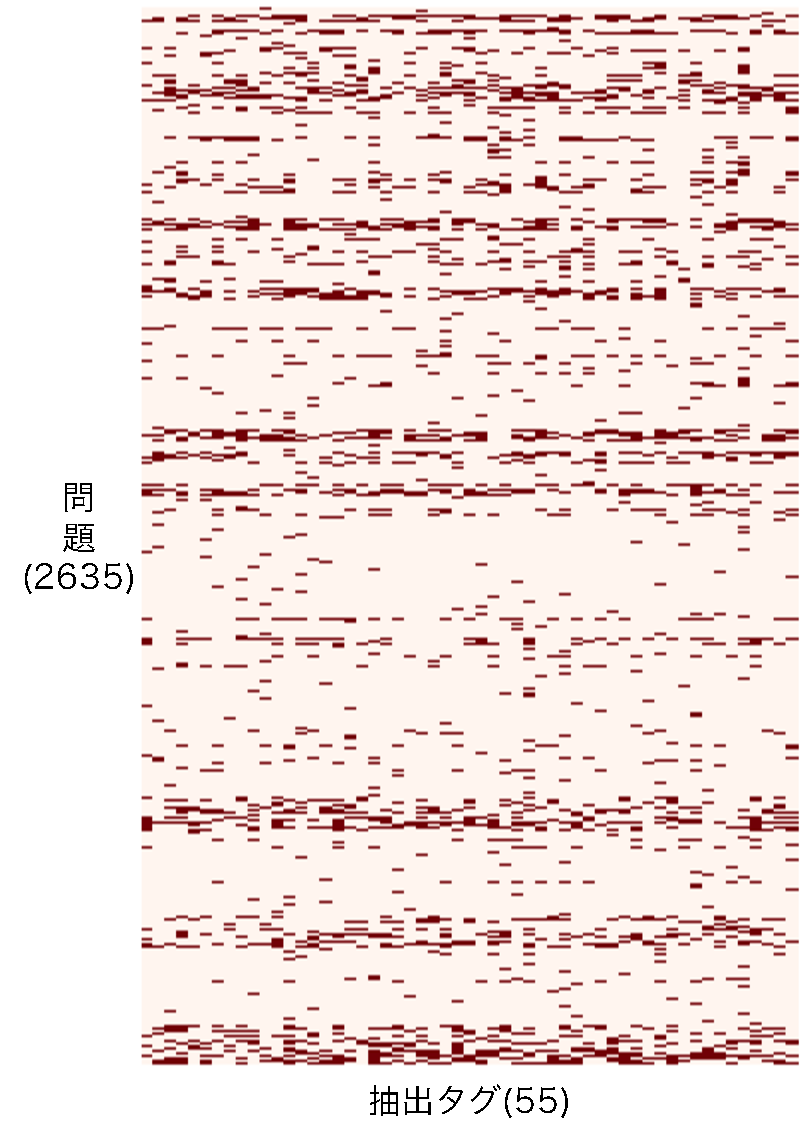
\includegraphics[height=180pt]{./img/aDiscrete.pdf}
		\subcaption{「ASSISTments 2009-2010」}
	\endminipage\hfill
	\minipage{0.55\textwidth}
		\centering
		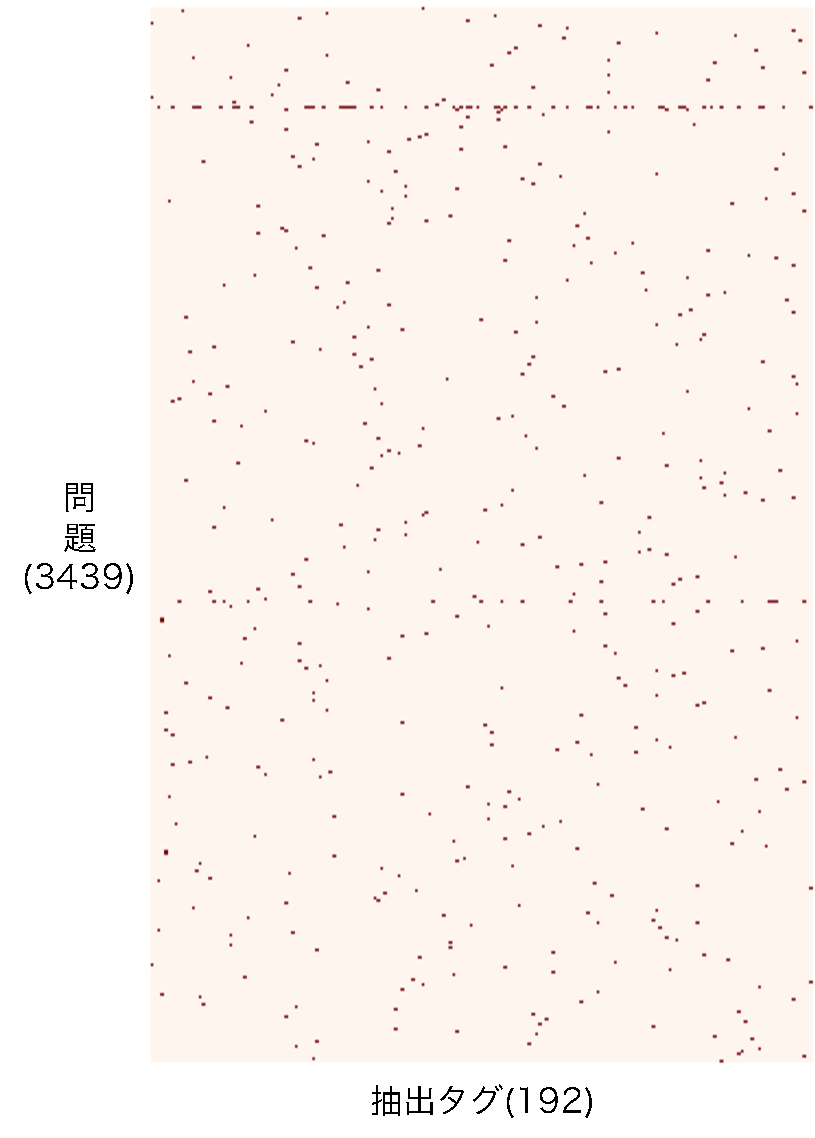
\includegraphics[height=180pt]{./img/kDiscrete.pdf}
		\subcaption{「Bridge to Algebra 2006-2007」}
	\endminipage\hfill
}
\end{center}
\caption{問題と抽出タグの関係性}
\label{fig:Discrete}
\end{figure}


次に,上記の行列と既存の知識分類から,抽出タグと既存タグの問題を媒介とする共起行列を作成してヒートマップとして可視化し,
さらに各既存タグが回答ログにおいて出現する回数をグラフ化したものを
合わせたものを図\ref{fig:Heatmap}に表す.
%まず,抽出タグと既存タグの問題を媒介とする共起行列をヒートマップとして可視化したものを図\ref{fig:aHeatmap}, \ref{fig:kHeatmap}, に表す.
ヒートマップ上で赤色が濃い成分ほど値が大きく,薄い成分ほど値が小さく,
各行が抽出タグを,各列が既存タグを表しており,
ヒートマップ上部のグラフの横軸はヒートマップの各列と対応している.
各列に対応する既存タグの名称はそれぞれ図\ref{fig:aTable3},\ref{fig:kTable3}のとおりである.
図から,回答ログにおける出現回数が多い既存タグは,多くの抽出タグにおいて強く共起しており,
出現回数が少ないタグは,少数の抽出タグのみと共起している.
%列番号に対応する既存タグの名称はヒートマップ横の表に掲載した.

\begin{figure}[H]
\begin{center}
\hspace*{-20pt}
\makebox[1.1\textwidth][c]{
	\minipage{0.55\textwidth}
		\centering
		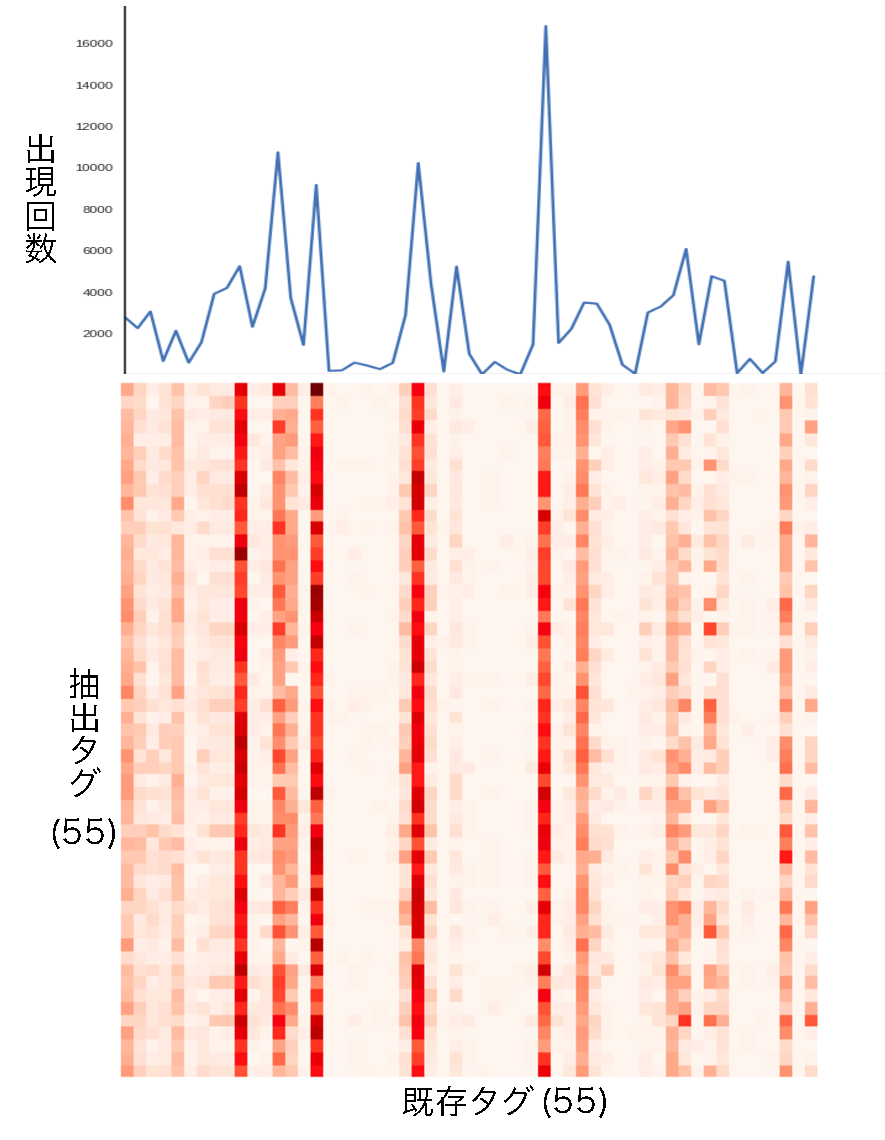
\includegraphics[height=260pt]{./img/aHeatmapGraph.pdf}
		\subcaption{「ASSISTments 2009-2010」}
	\endminipage\hfill
	\minipage{0.55\textwidth}
		\centering
		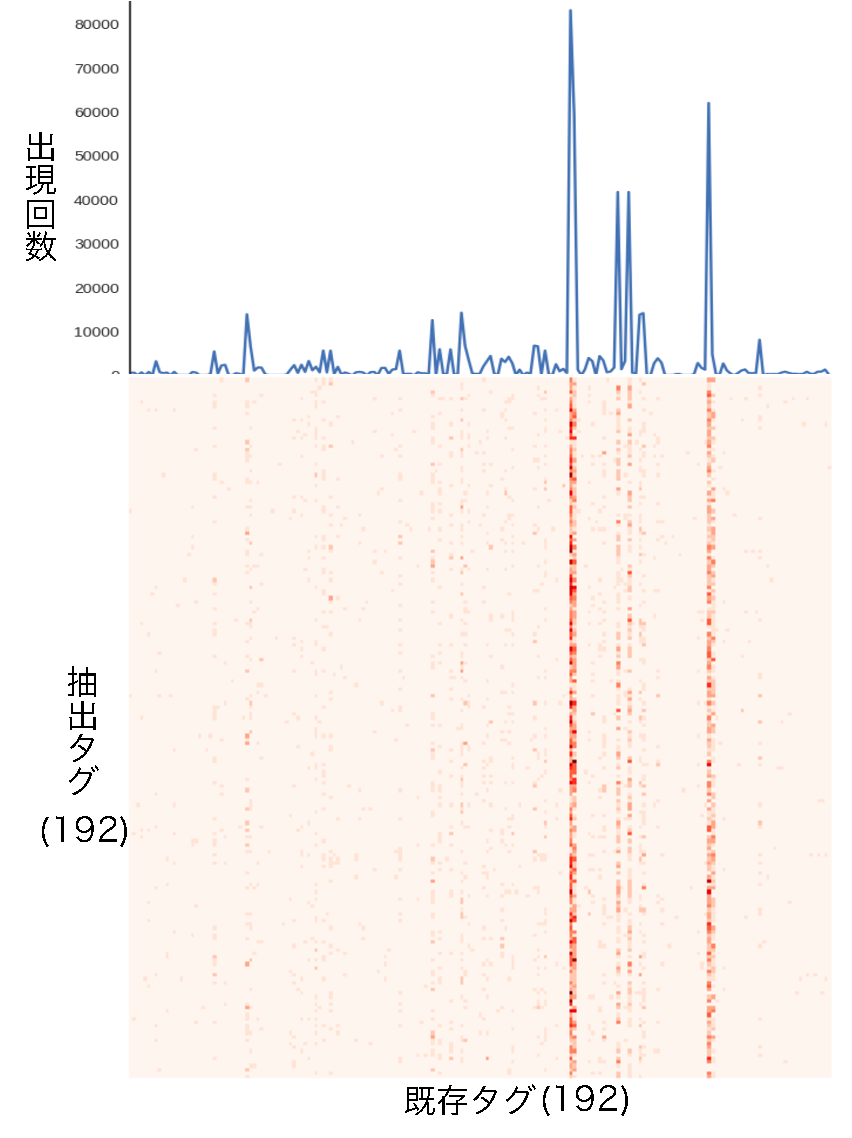
\includegraphics[height=260pt]{./img/kHeatmapGraph.pdf}
		\subcaption{「Bridge to Algebra 2006-2007」}
	\endminipage\hfill
}
\end{center}
\caption{抽出タグと既存タグの共起行列のヒートマップと各既存タグの出現回数のグラフ}
\label{fig:Heatmap}
\end{figure}


上記の共起行列を正規化して作成したタグ関係行列のヒートマップを図\ref{fig:Normalized}に表す.

\begin{figure}[H]
\begin{center}
\hspace*{-20pt}
\makebox[1.1\textwidth][c]{
	\minipage{0.55\textwidth}
		\centering
		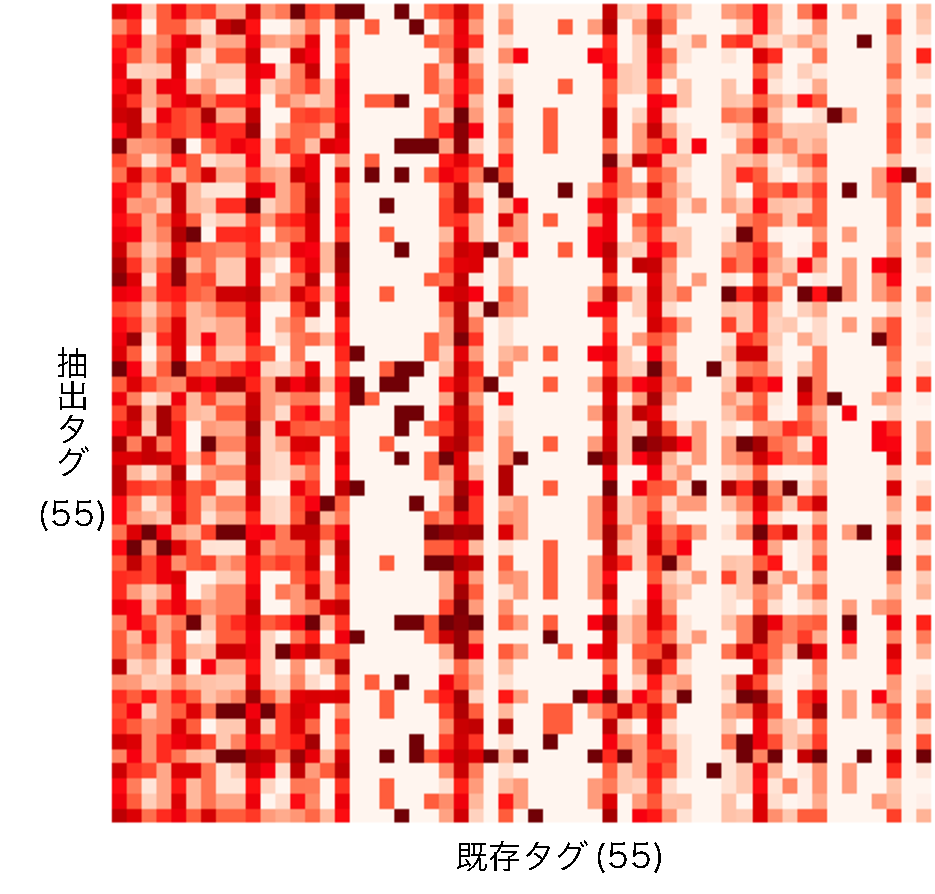
\includegraphics[height=220pt]{./img/aNormalized.pdf}
		\subcaption{「ASSISTments 2009-2010」}
	\endminipage\hfill
	\minipage{0.55\textwidth}
		\centering
		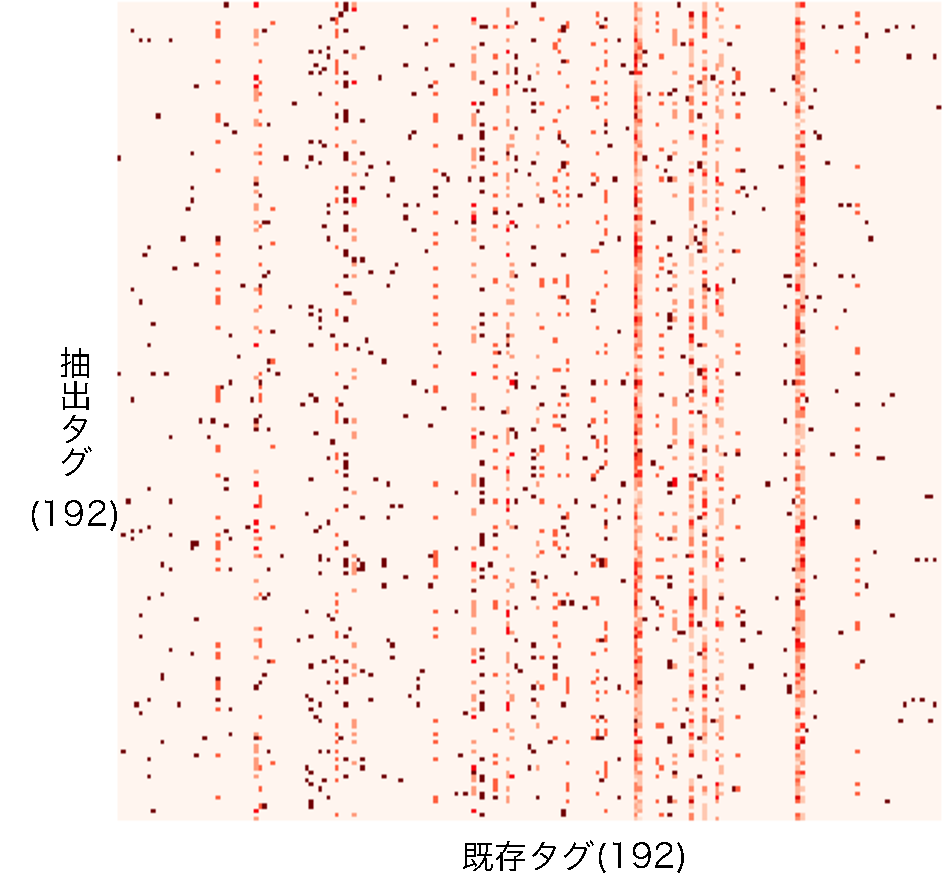
\includegraphics[height=220pt]{./img/kNormalized.pdf}
		\subcaption{「Bridge to Algebra 2006-2007」}
	\endminipage\hfill
}
\end{center}
\caption{タグ関係行列のヒートマップ}
\label{fig:Normalized}
\end{figure}

既存タグの知識間影響ネットワークである既存タグネットワークの概形を図\ref{fig:SimpleNetwork}に,
既存タグネットワークとタグ関係行列から作成した,抽出タグと既存タグの関係性を表すタグ関係ネットワークの概形を図\ref{fig:Network}に表す.
%なお,タグ関係ネットワークにおいて接続している抽出タグと既存タグの組み合わせは付録にまとめた.

\begin{figure}[H]
\begin{center}
\hspace*{-20pt}
\makebox[1.1\textwidth][c]{
	\minipage{0.55\textwidth}
		\centering
		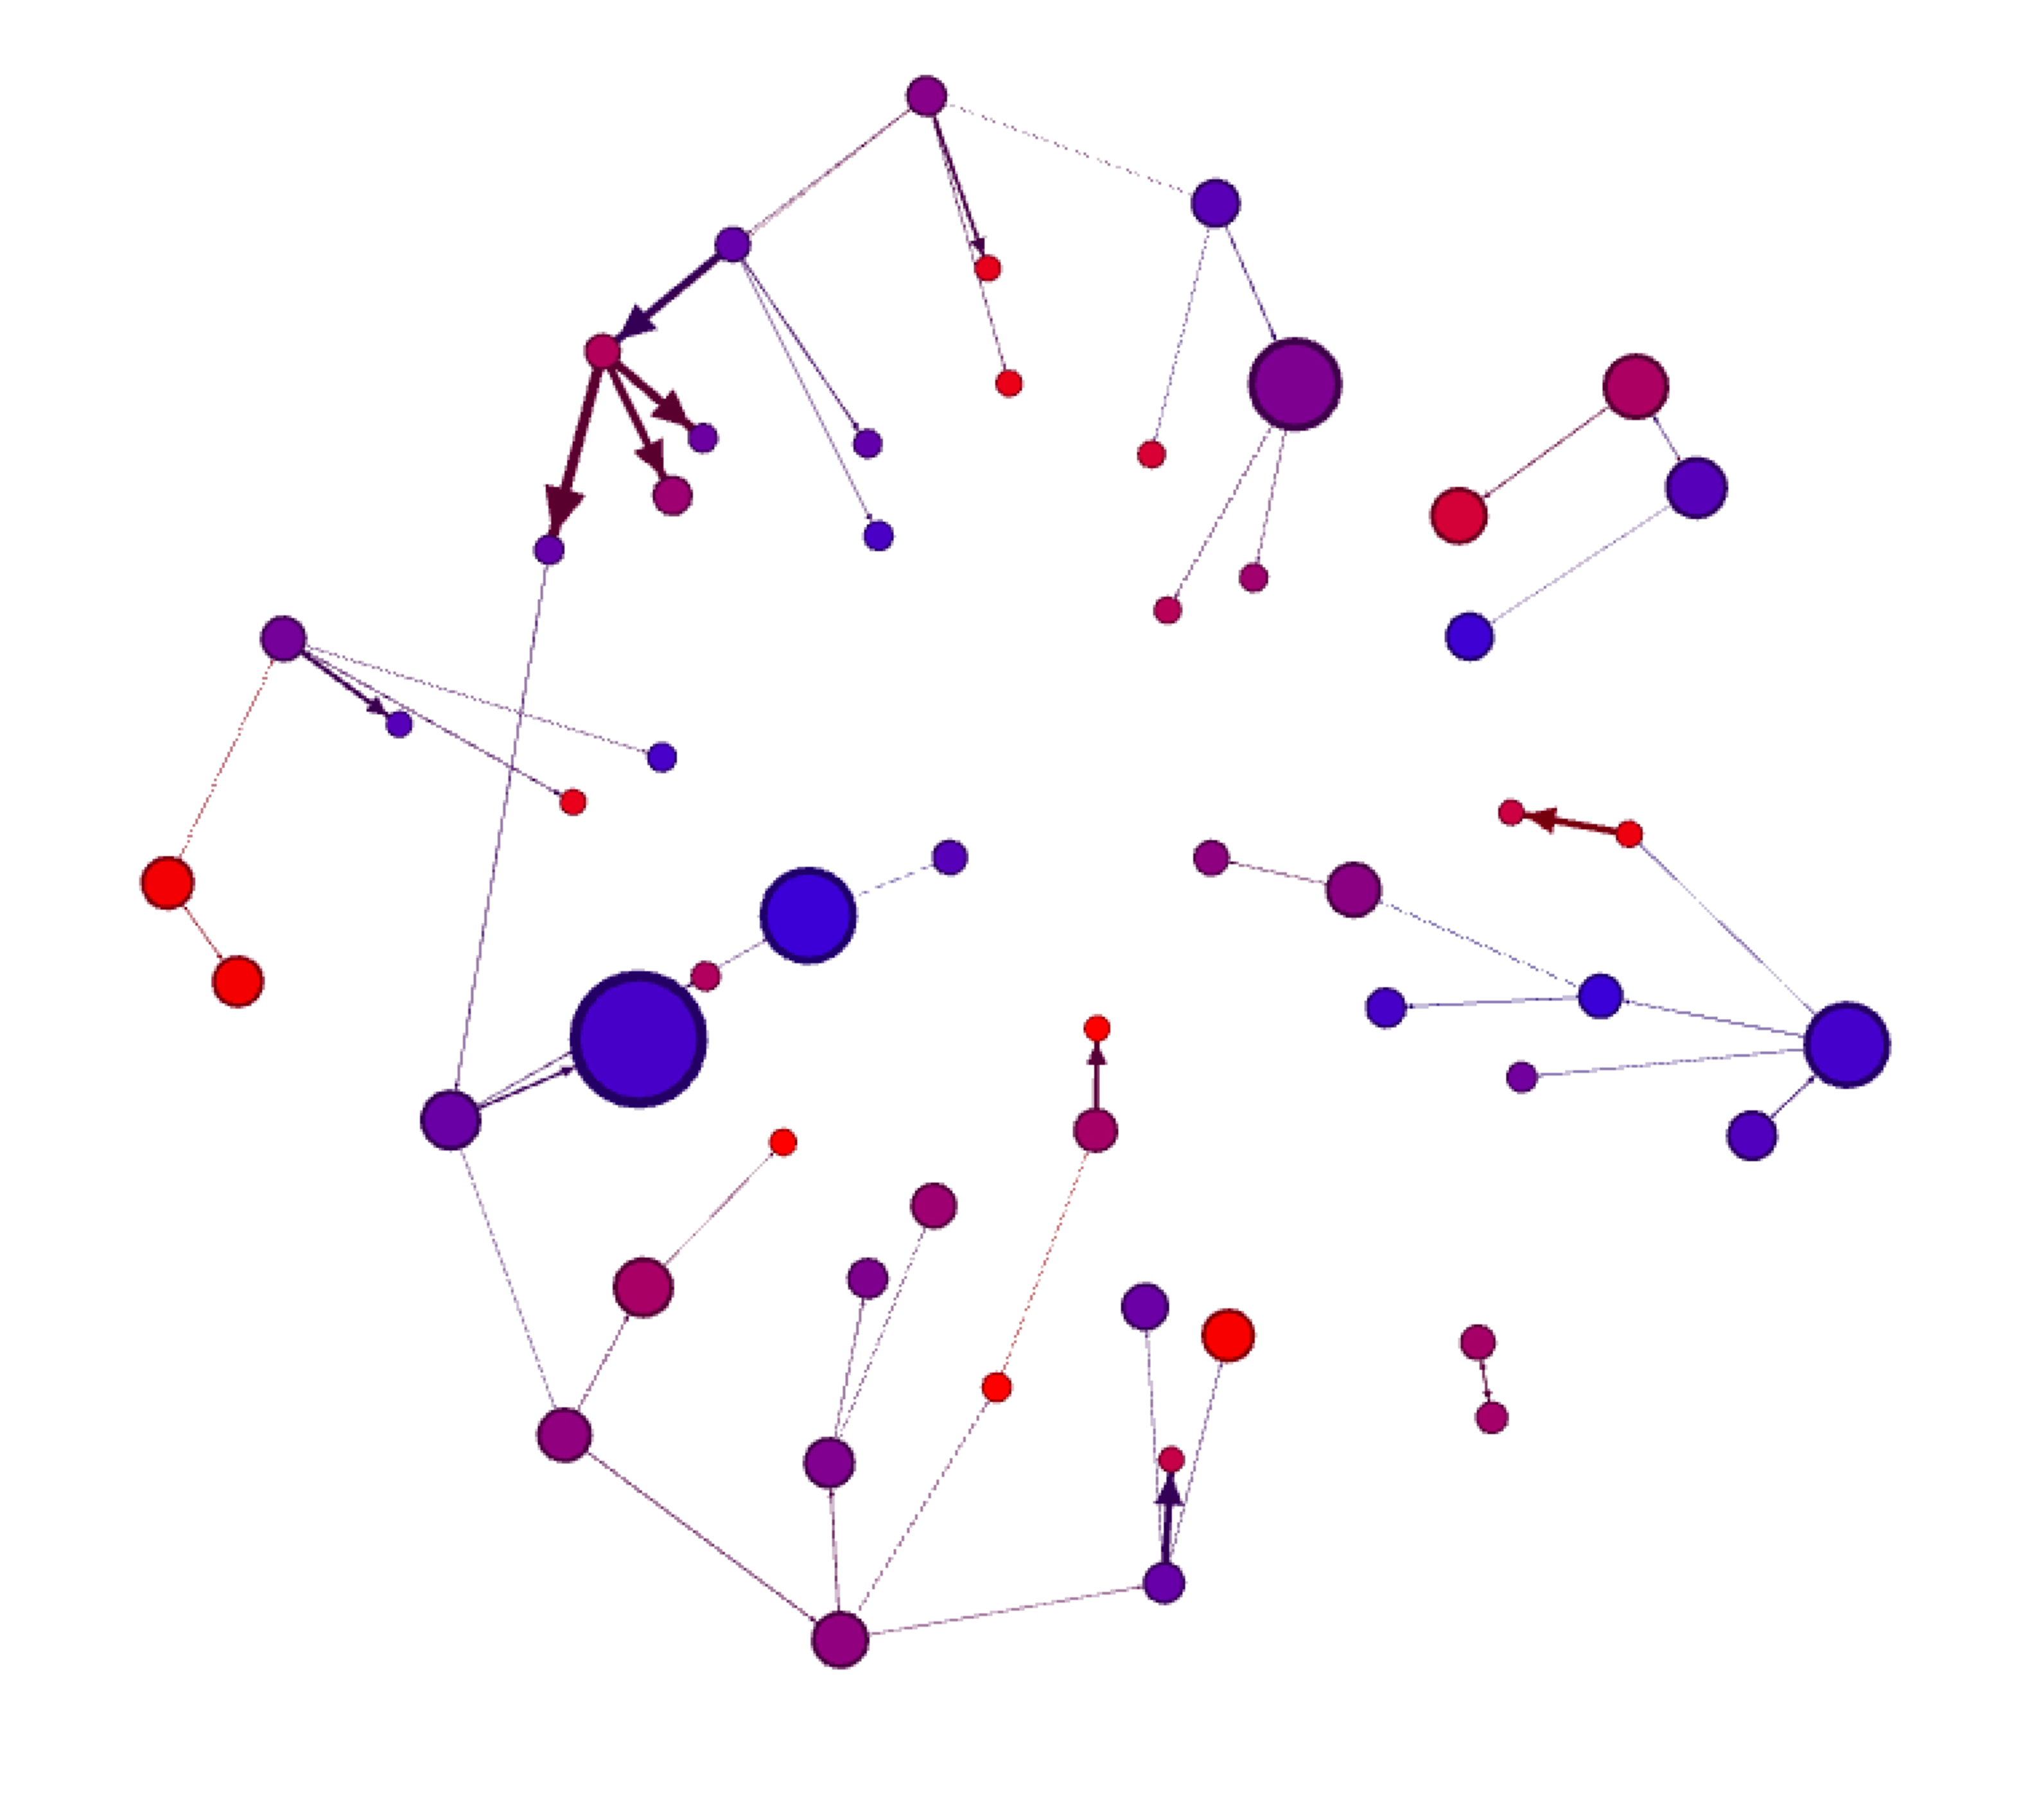
\includegraphics[height=220pt]{./img/aSimpleNetwork2.pdf}
		\subcaption{「ASSISTments 2009-2010」}
	\endminipage\hfill
	\minipage{0.55\textwidth}
		\centering
		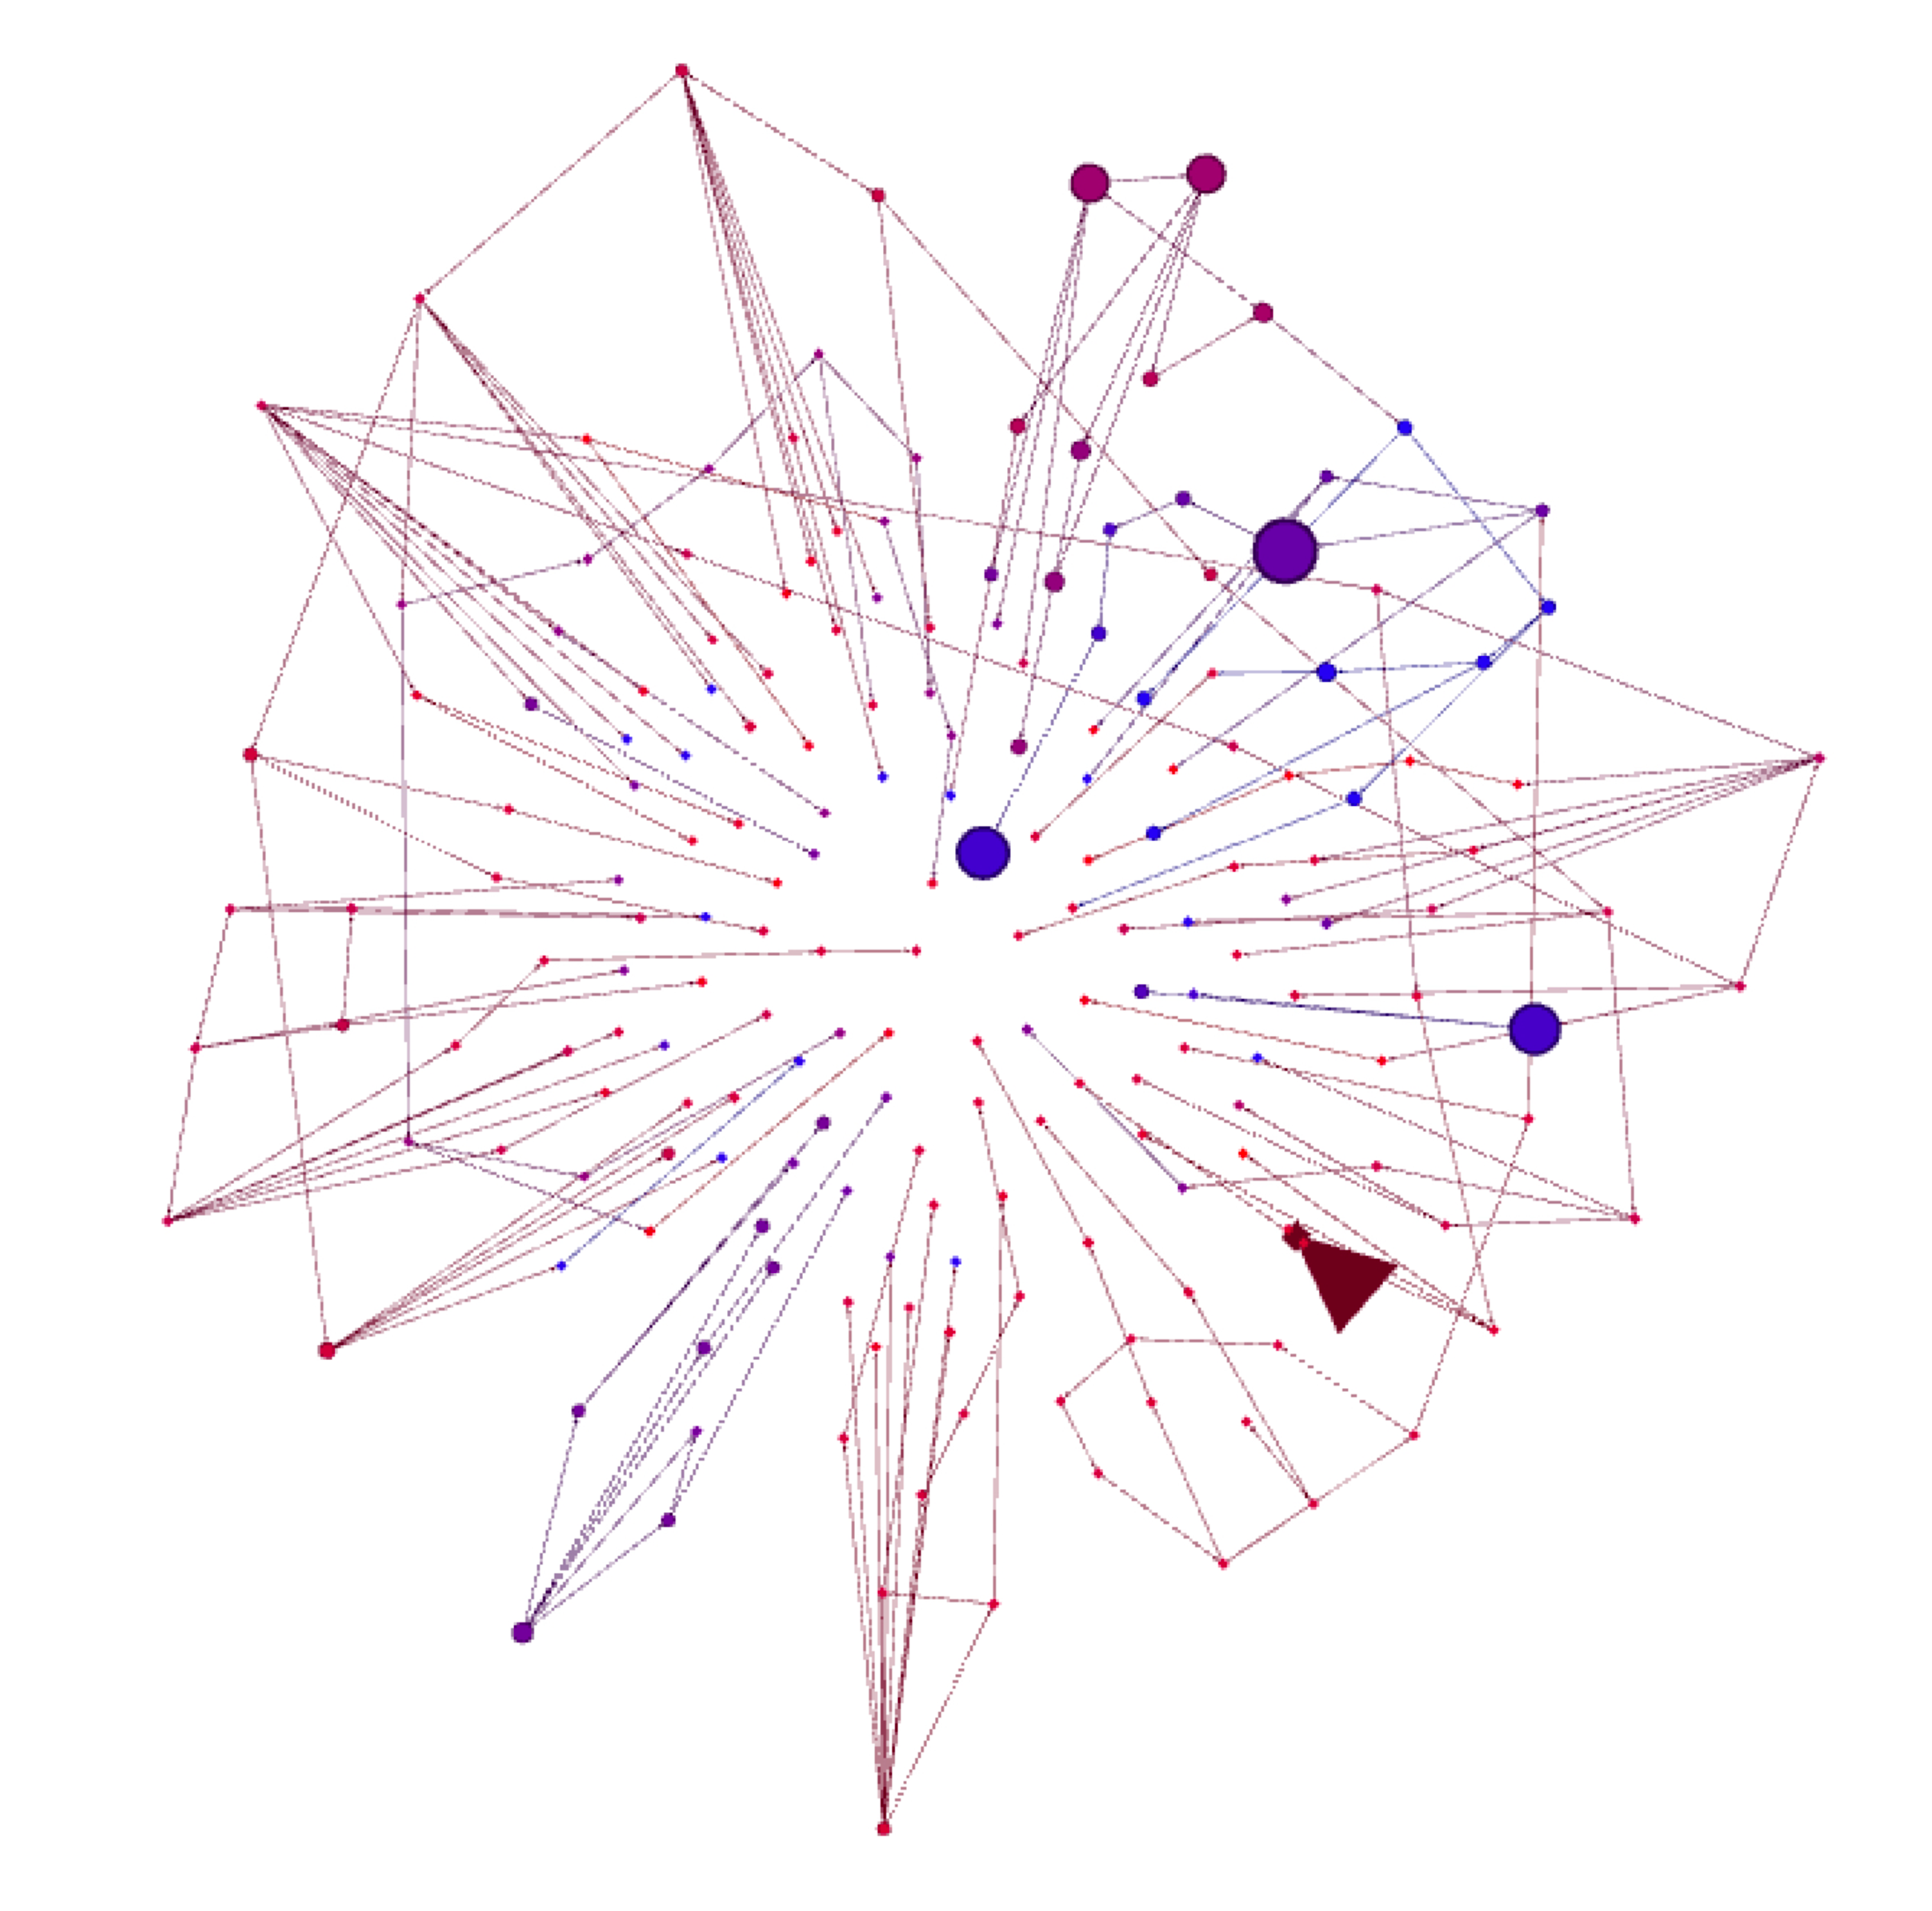
\includegraphics[height=220pt]{./img/kSimpleNetwork2.pdf}
		\subcaption{「Bridge to Algebra 2006-2007」}
	\endminipage\hfill
}
\end{center}
\caption{既存タグネットワークの構造}
\label{fig:SimpleNetwork}
\end{figure}

\begin{figure}[H]
\begin{center}
\hspace*{-20pt}
\makebox[1.1\textwidth][c]{
	\minipage{0.55\textwidth}
		\centering
		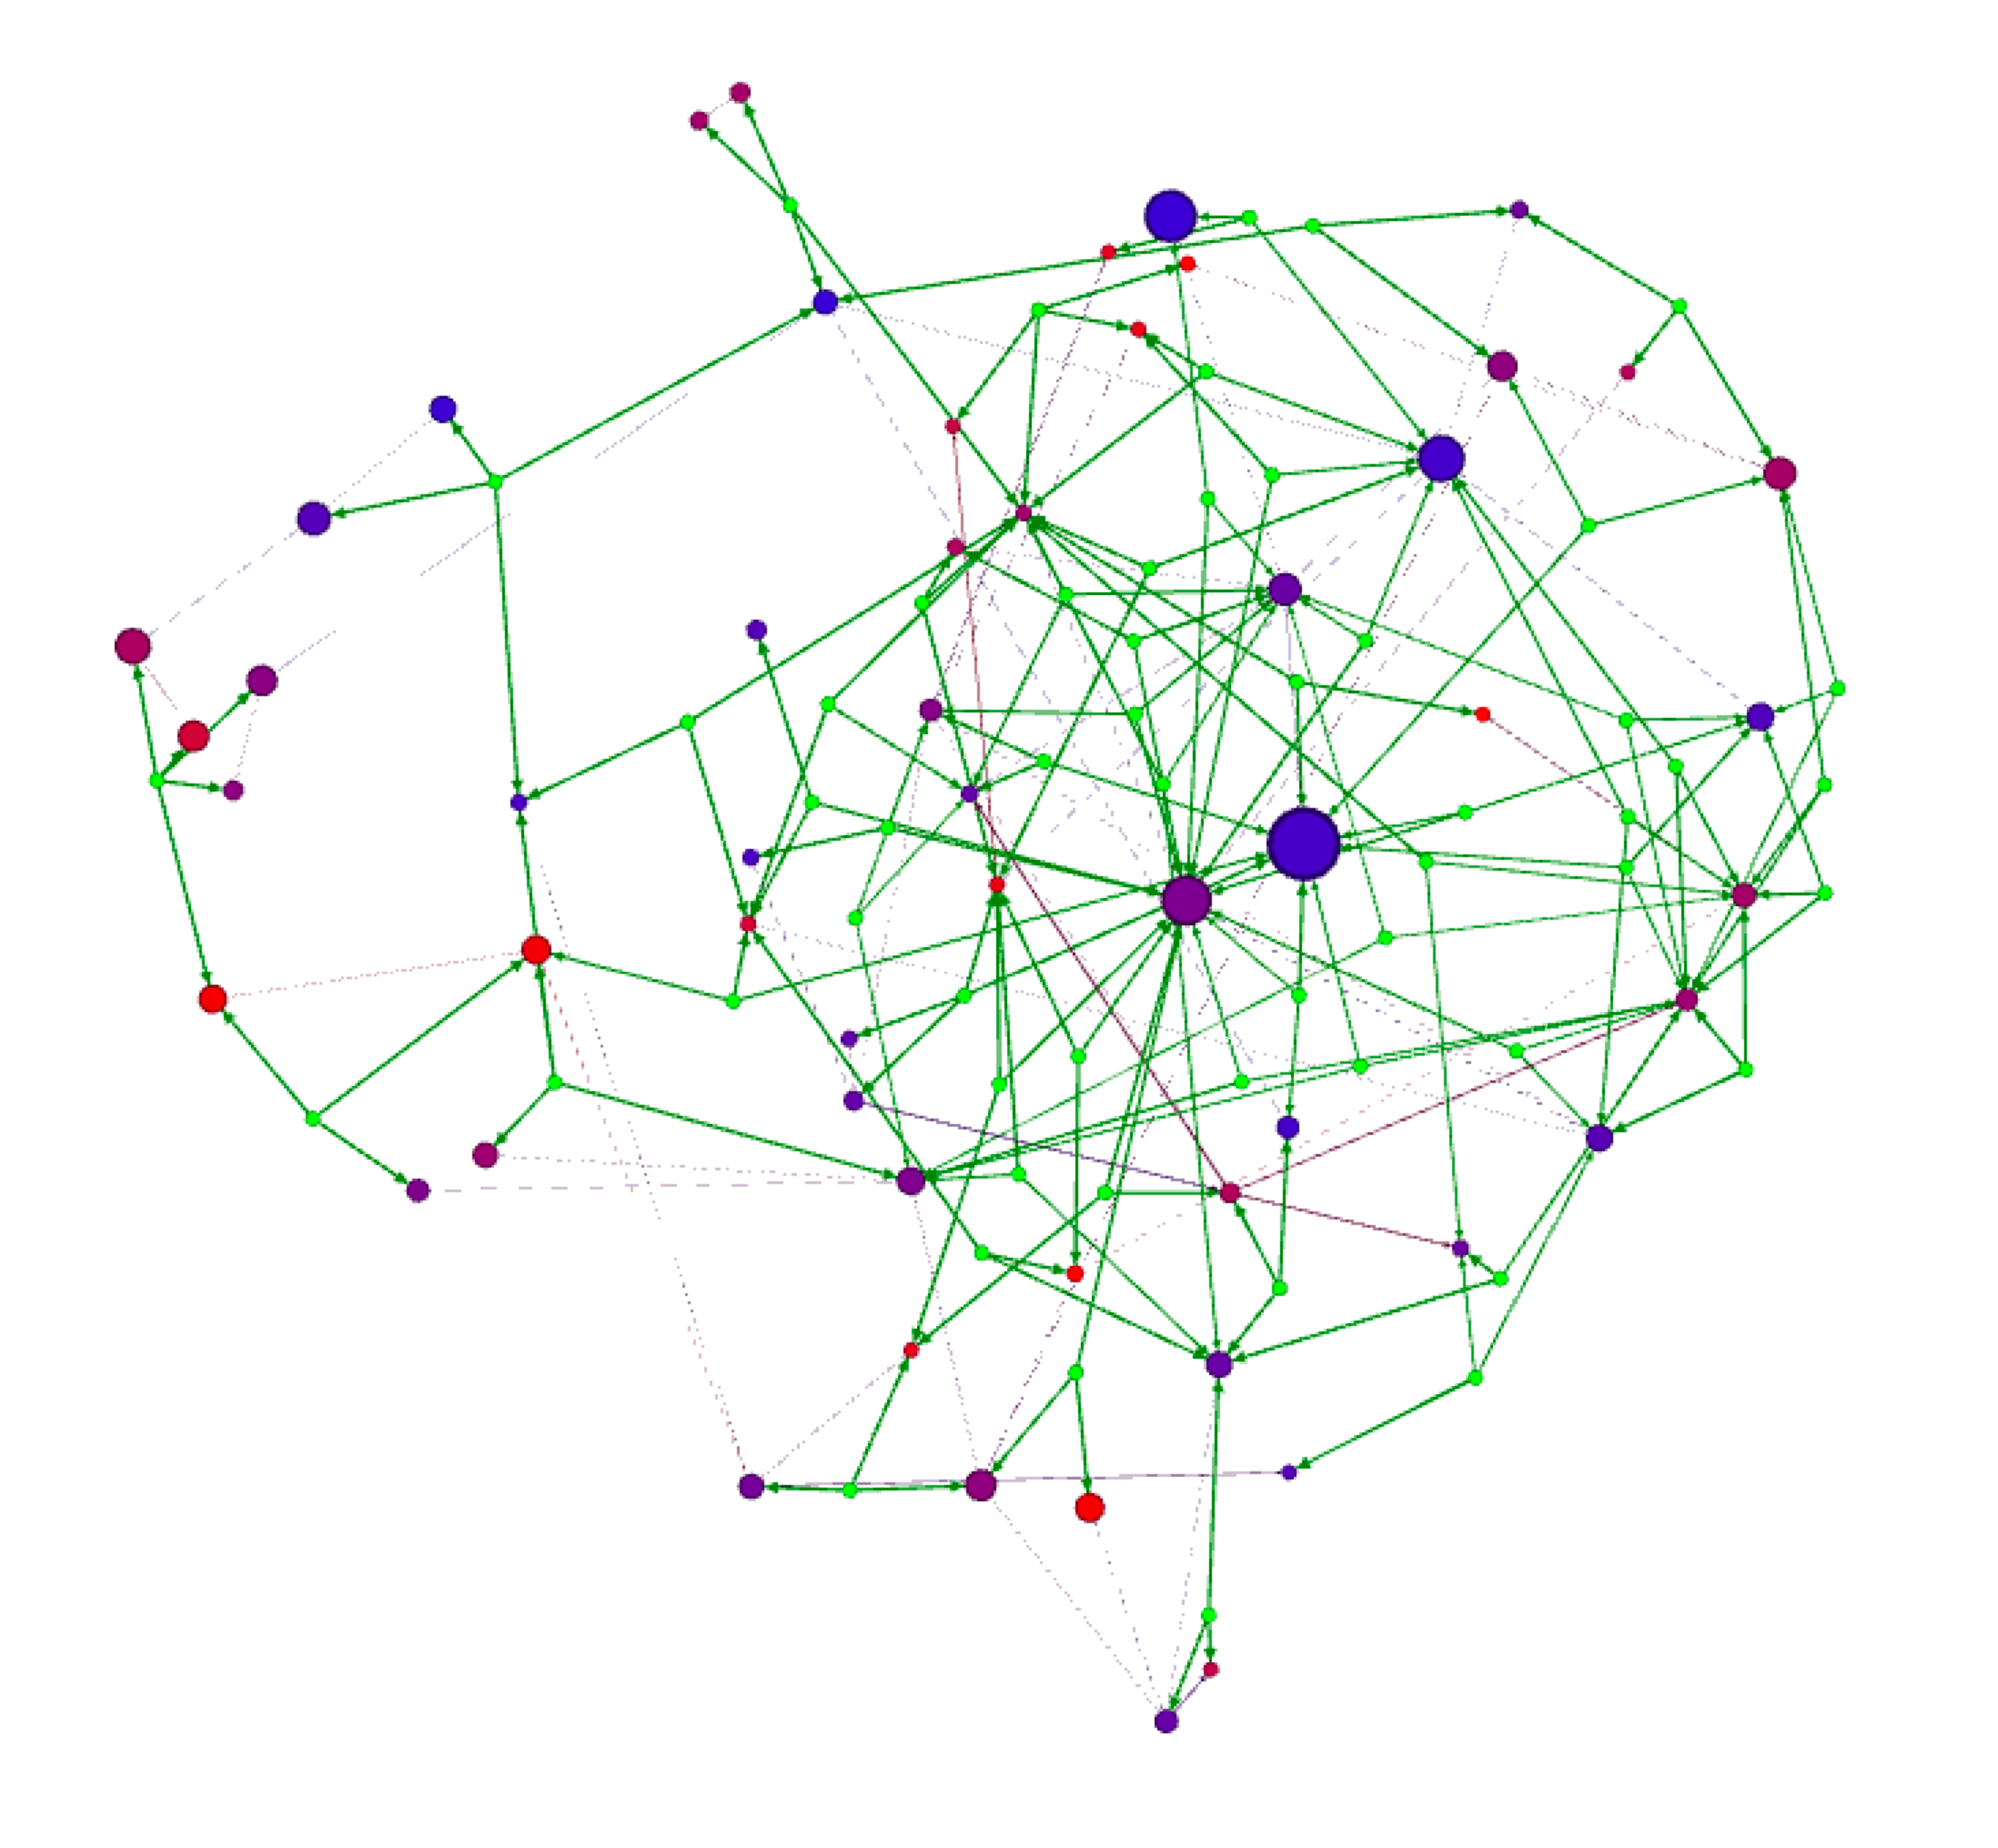
\includegraphics[height=220pt]{./img/aNetwork2.pdf}
		\subcaption{「ASSISTments 2009-2010」}
	\endminipage\hfill
	\minipage{0.55\textwidth}
		\centering
		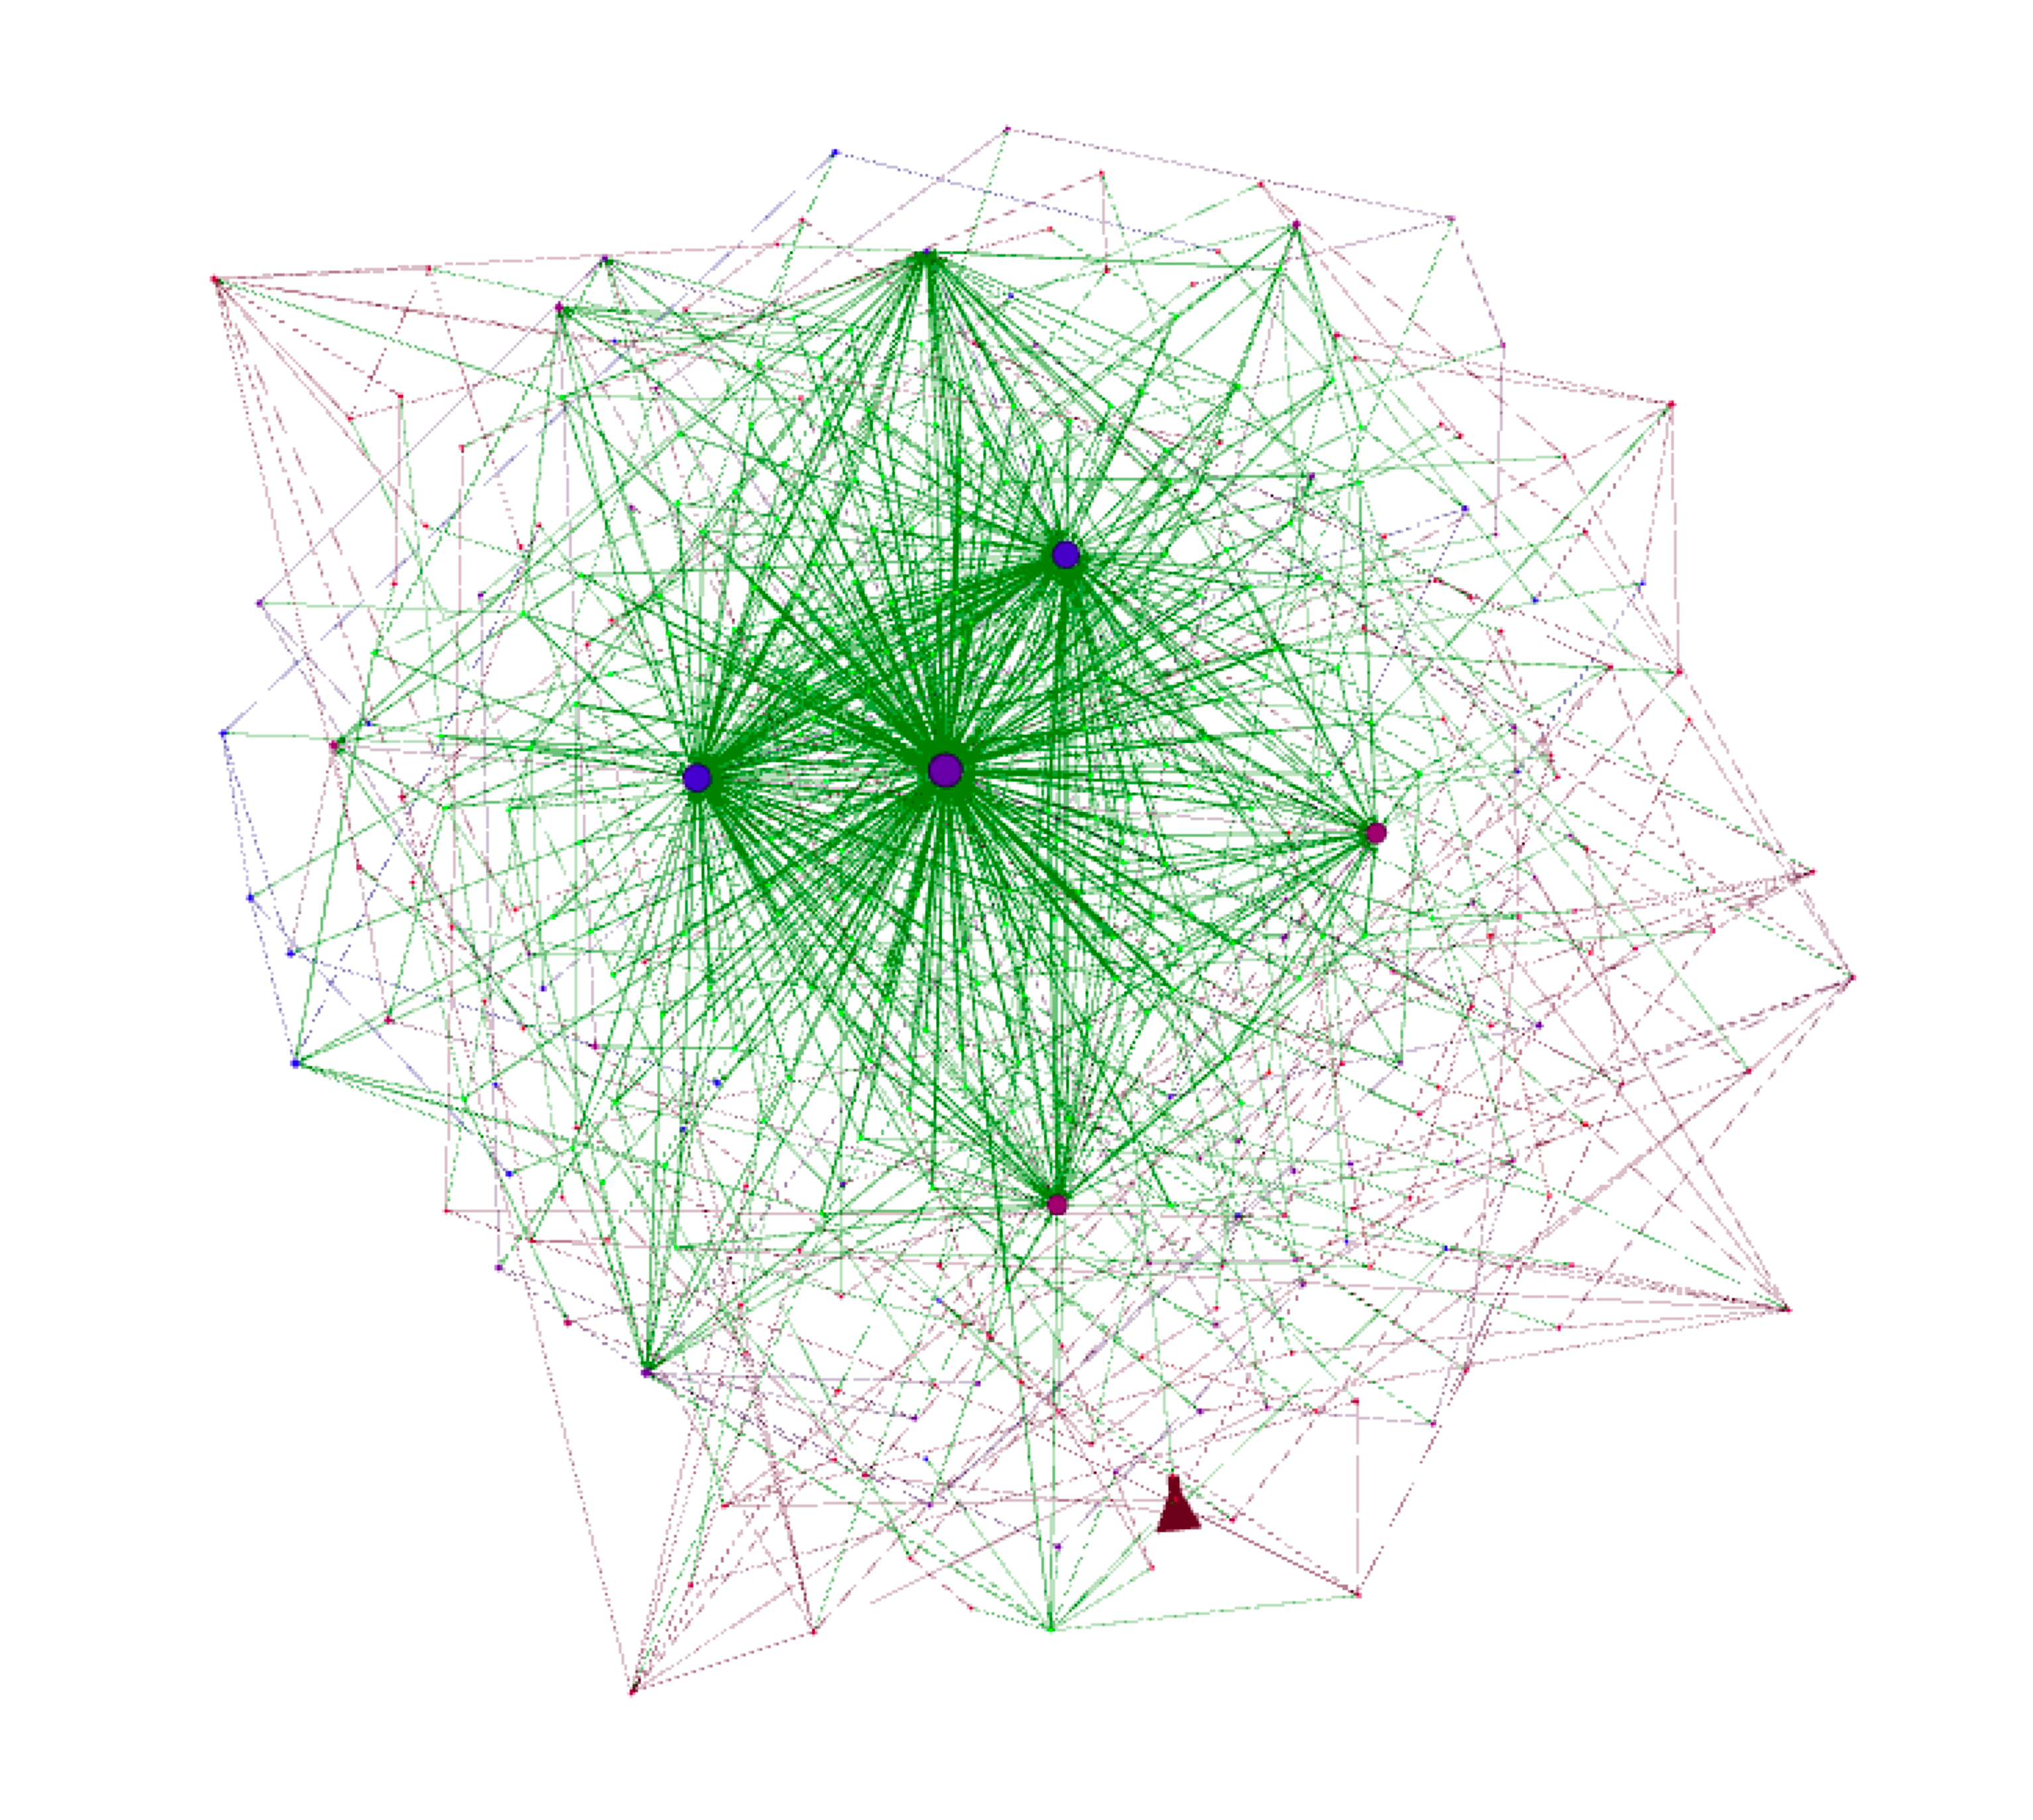
\includegraphics[height=220pt]{./img/kNetwork2.pdf}
		\subcaption{「Bridge to Algebra 2006-2007」}
	\endminipage\hfill
}
\end{center}
\caption{タグ関係ネットワークの構造}
\label{fig:Network}
\end{figure}




\subsection{抽出タグと既存タグの比較分析}
抽出タグを既存タグと比較することにより,
抽出タグの性質を定量的・定性的に分析する.



まず,知識獲得予測の精度を向上させる要因を,データの構造から分析した.
抽出タグと既存タグそれぞれにおいて,各タグが回答ログに出現する回数の分布の比較と,各分布の標準偏差$\sigma$を図\ref{fig:AppearHist}に表す.
図より,既存タグはタグごとの出現回数の分散が大きい一方で,
抽出タグは分散が小さく,特定の値の周辺に集中していることがわかる.
この分布の違いと予測精度の関係性については,第6章で考察する.


\begin{figure}[htb]
\begin{center}
%\hspace*{-40pt}\makebox[1.2\textwidth][c]{
\hspace*{-20pt}\makebox[1.1\textwidth][c]{
	\minipage{0.53\textwidth}
		\centering
		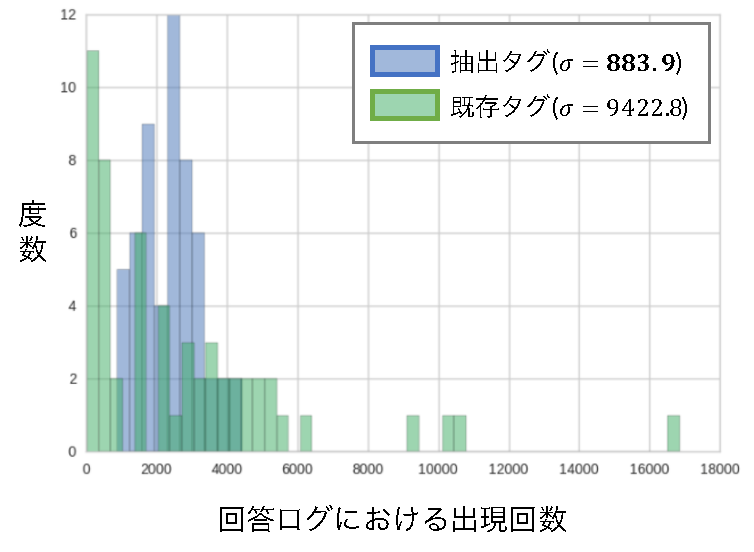
\includegraphics[width=180pt]{./img/aAppearHist.pdf}
		\subcaption{「ASSISTments 2009-2010」}
	\endminipage\hfill
	\minipage{0.53\textwidth}
		\centering
		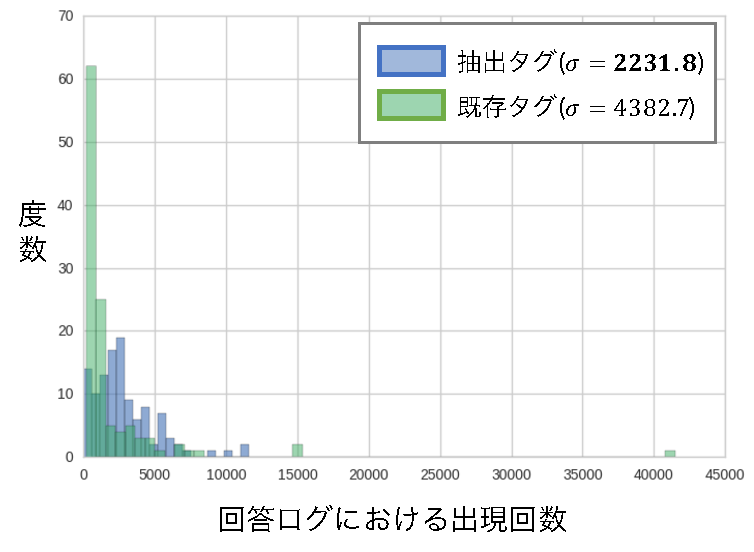
\includegraphics[width=180pt]{./img/kAppearHist.pdf}
		\subcaption{「Bridge to Algebra 2006-2007」}
	\endminipage\hfill
}
\end{center}
\caption{各タグの出現回数の分布}
\label{fig:AppearHist}
\end{figure}


次に,
図\ref{fig:Network}のネットワークの局所的な特性に着目し,抽出タグと既存タグの構造や内容の関係性が観測できる部分を示す.
まず,既存タグに注目し,各既存タグに抽出タグがどのように紐付いているかを観察すると,
出現回数の多い既存タグ(大きいノード)は多くの抽出タグ(緑のノード)が紐付いている(図\ref{fig:NetworkConcentrate})一方,
出現回数の少ない既存タグ(小さいノード)は特定の抽出タグのみ紐付き,多くは紐付いていない(図\ref{fig:NetworkLittle})ことがわかる.

\begin{figure}[htb]
\begin{center}
%\hspace*{-40pt}\makebox[1.2\textwidth][c]{
\hspace*{-20pt}\makebox[1.1\textwidth][c]{
	\minipage{0.53\textwidth}
		\centering
		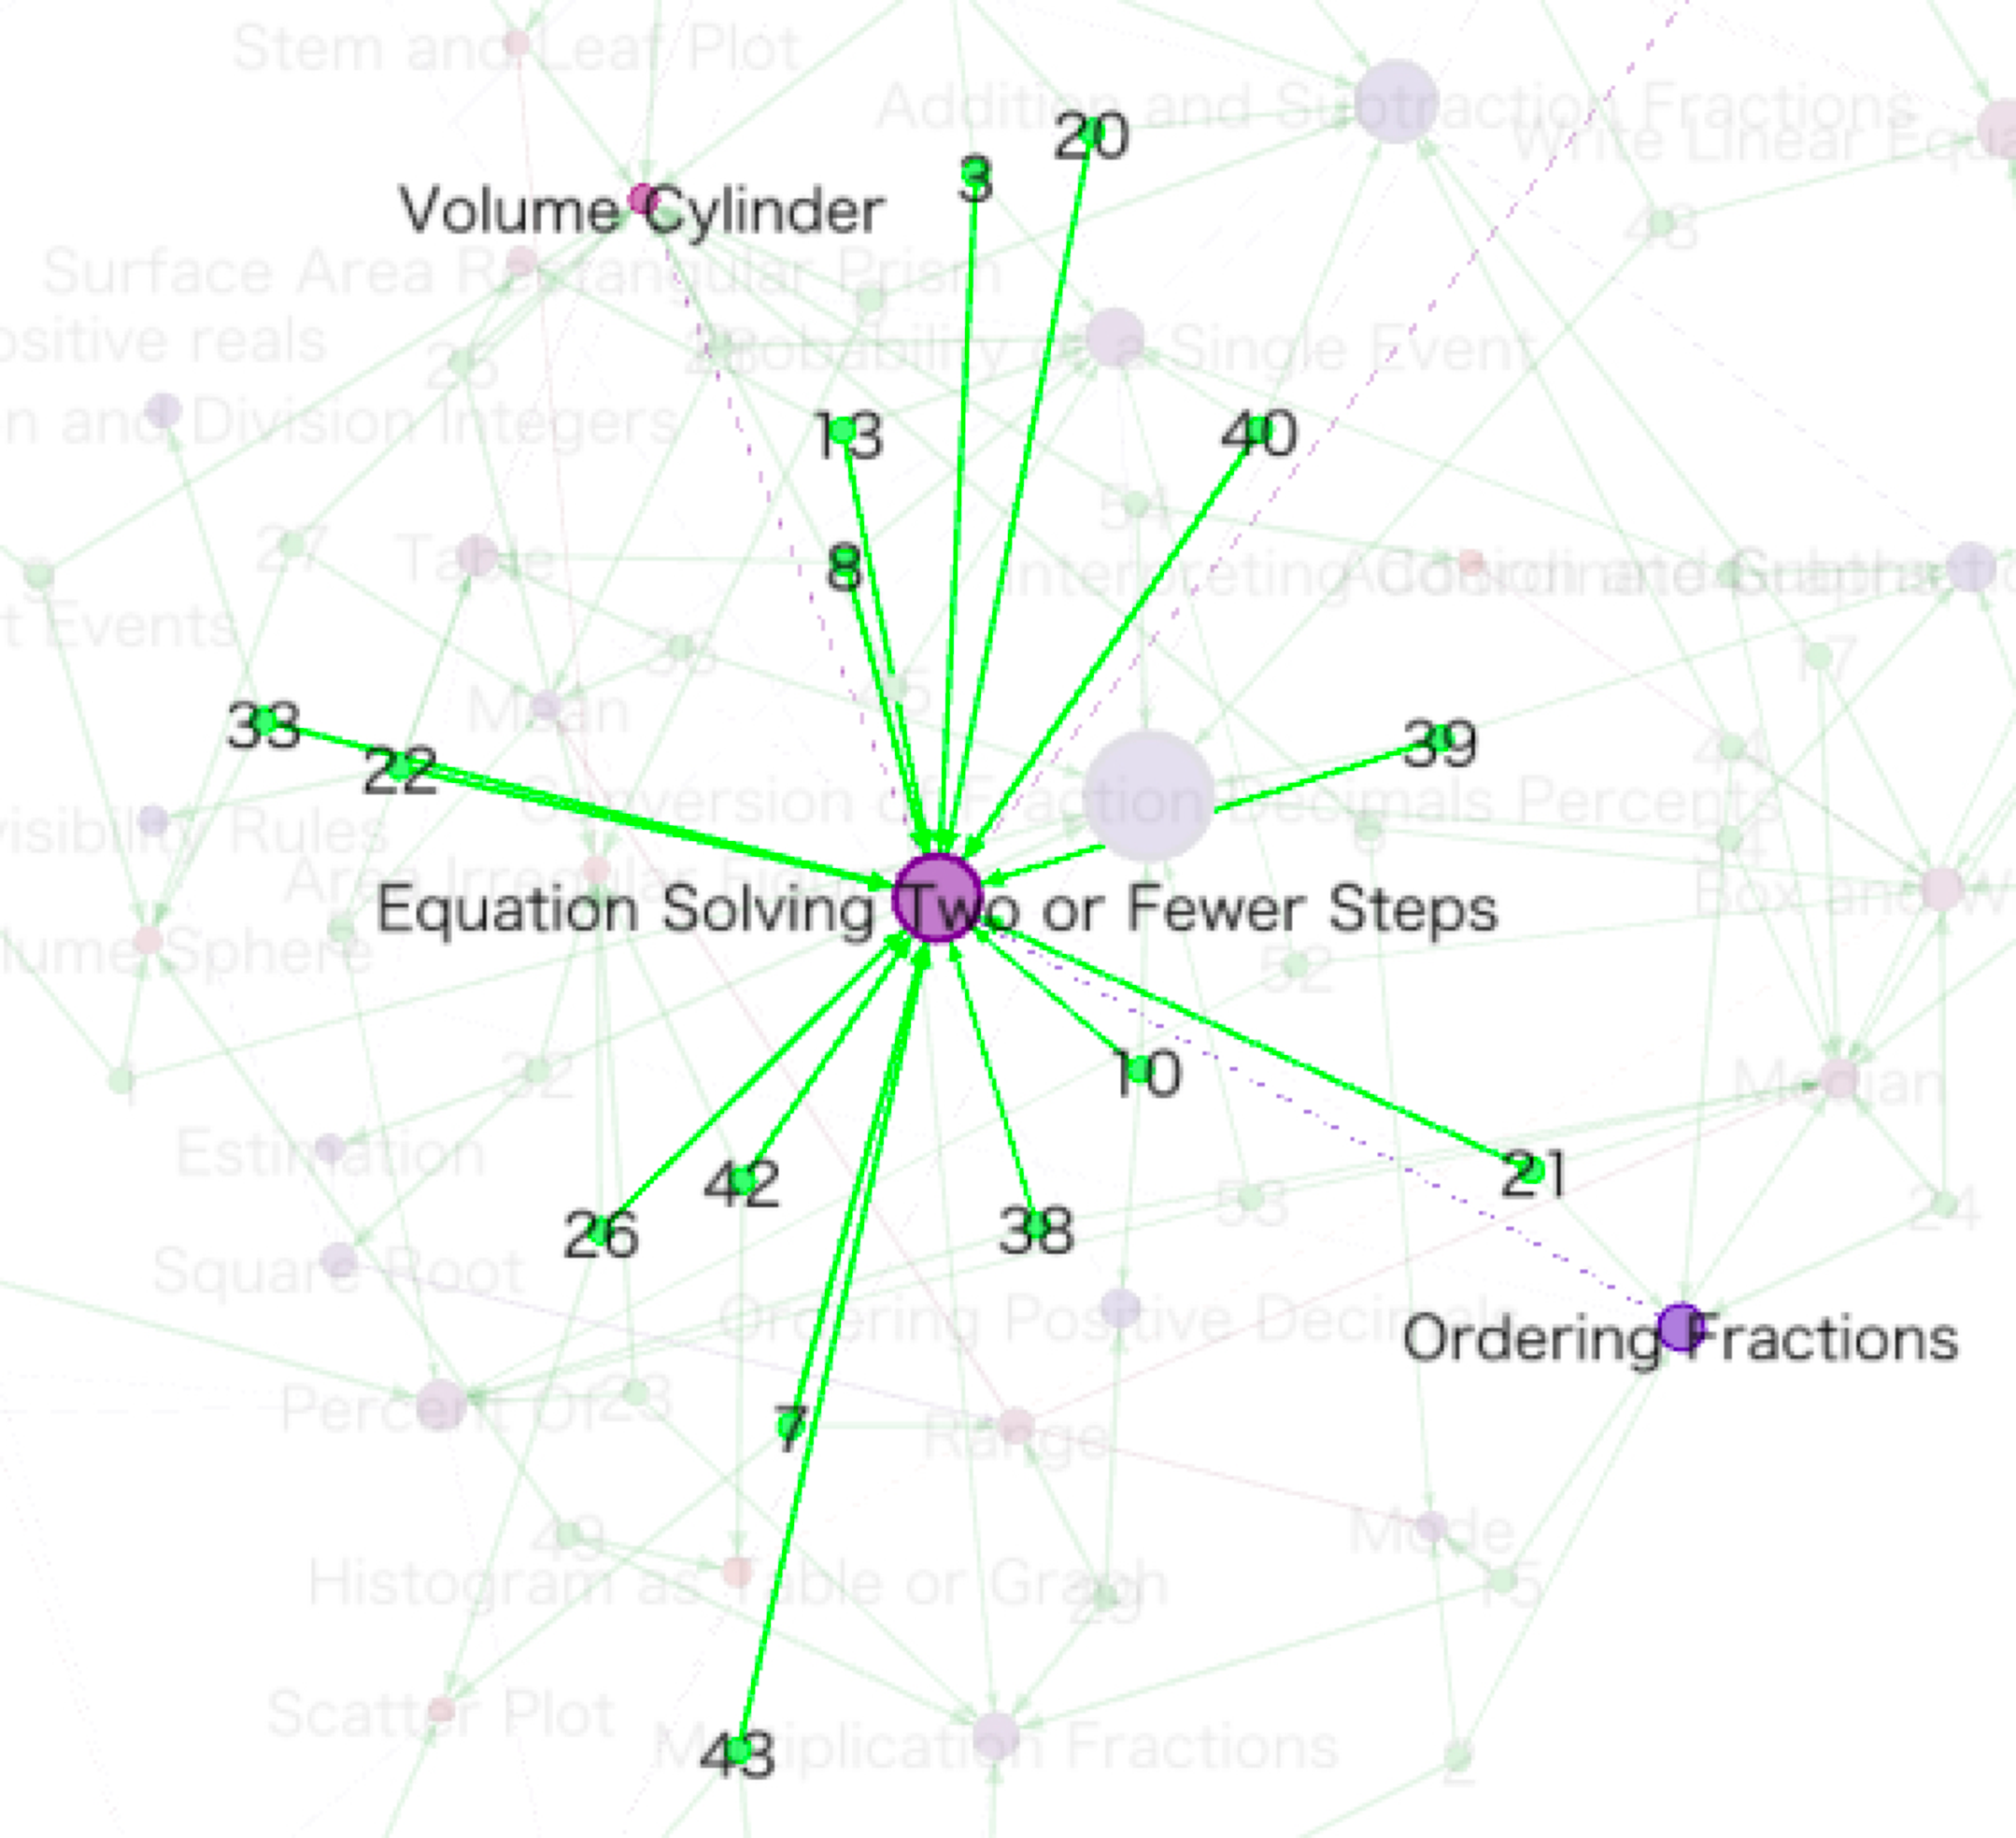
\includegraphics[height=120pt]{./img/aNetworkConcentrate2.pdf}
		\subcaption{「ASSISTments 2009-2010」}
	\endminipage\hfill
	\minipage{0.53\textwidth}
		\centering
		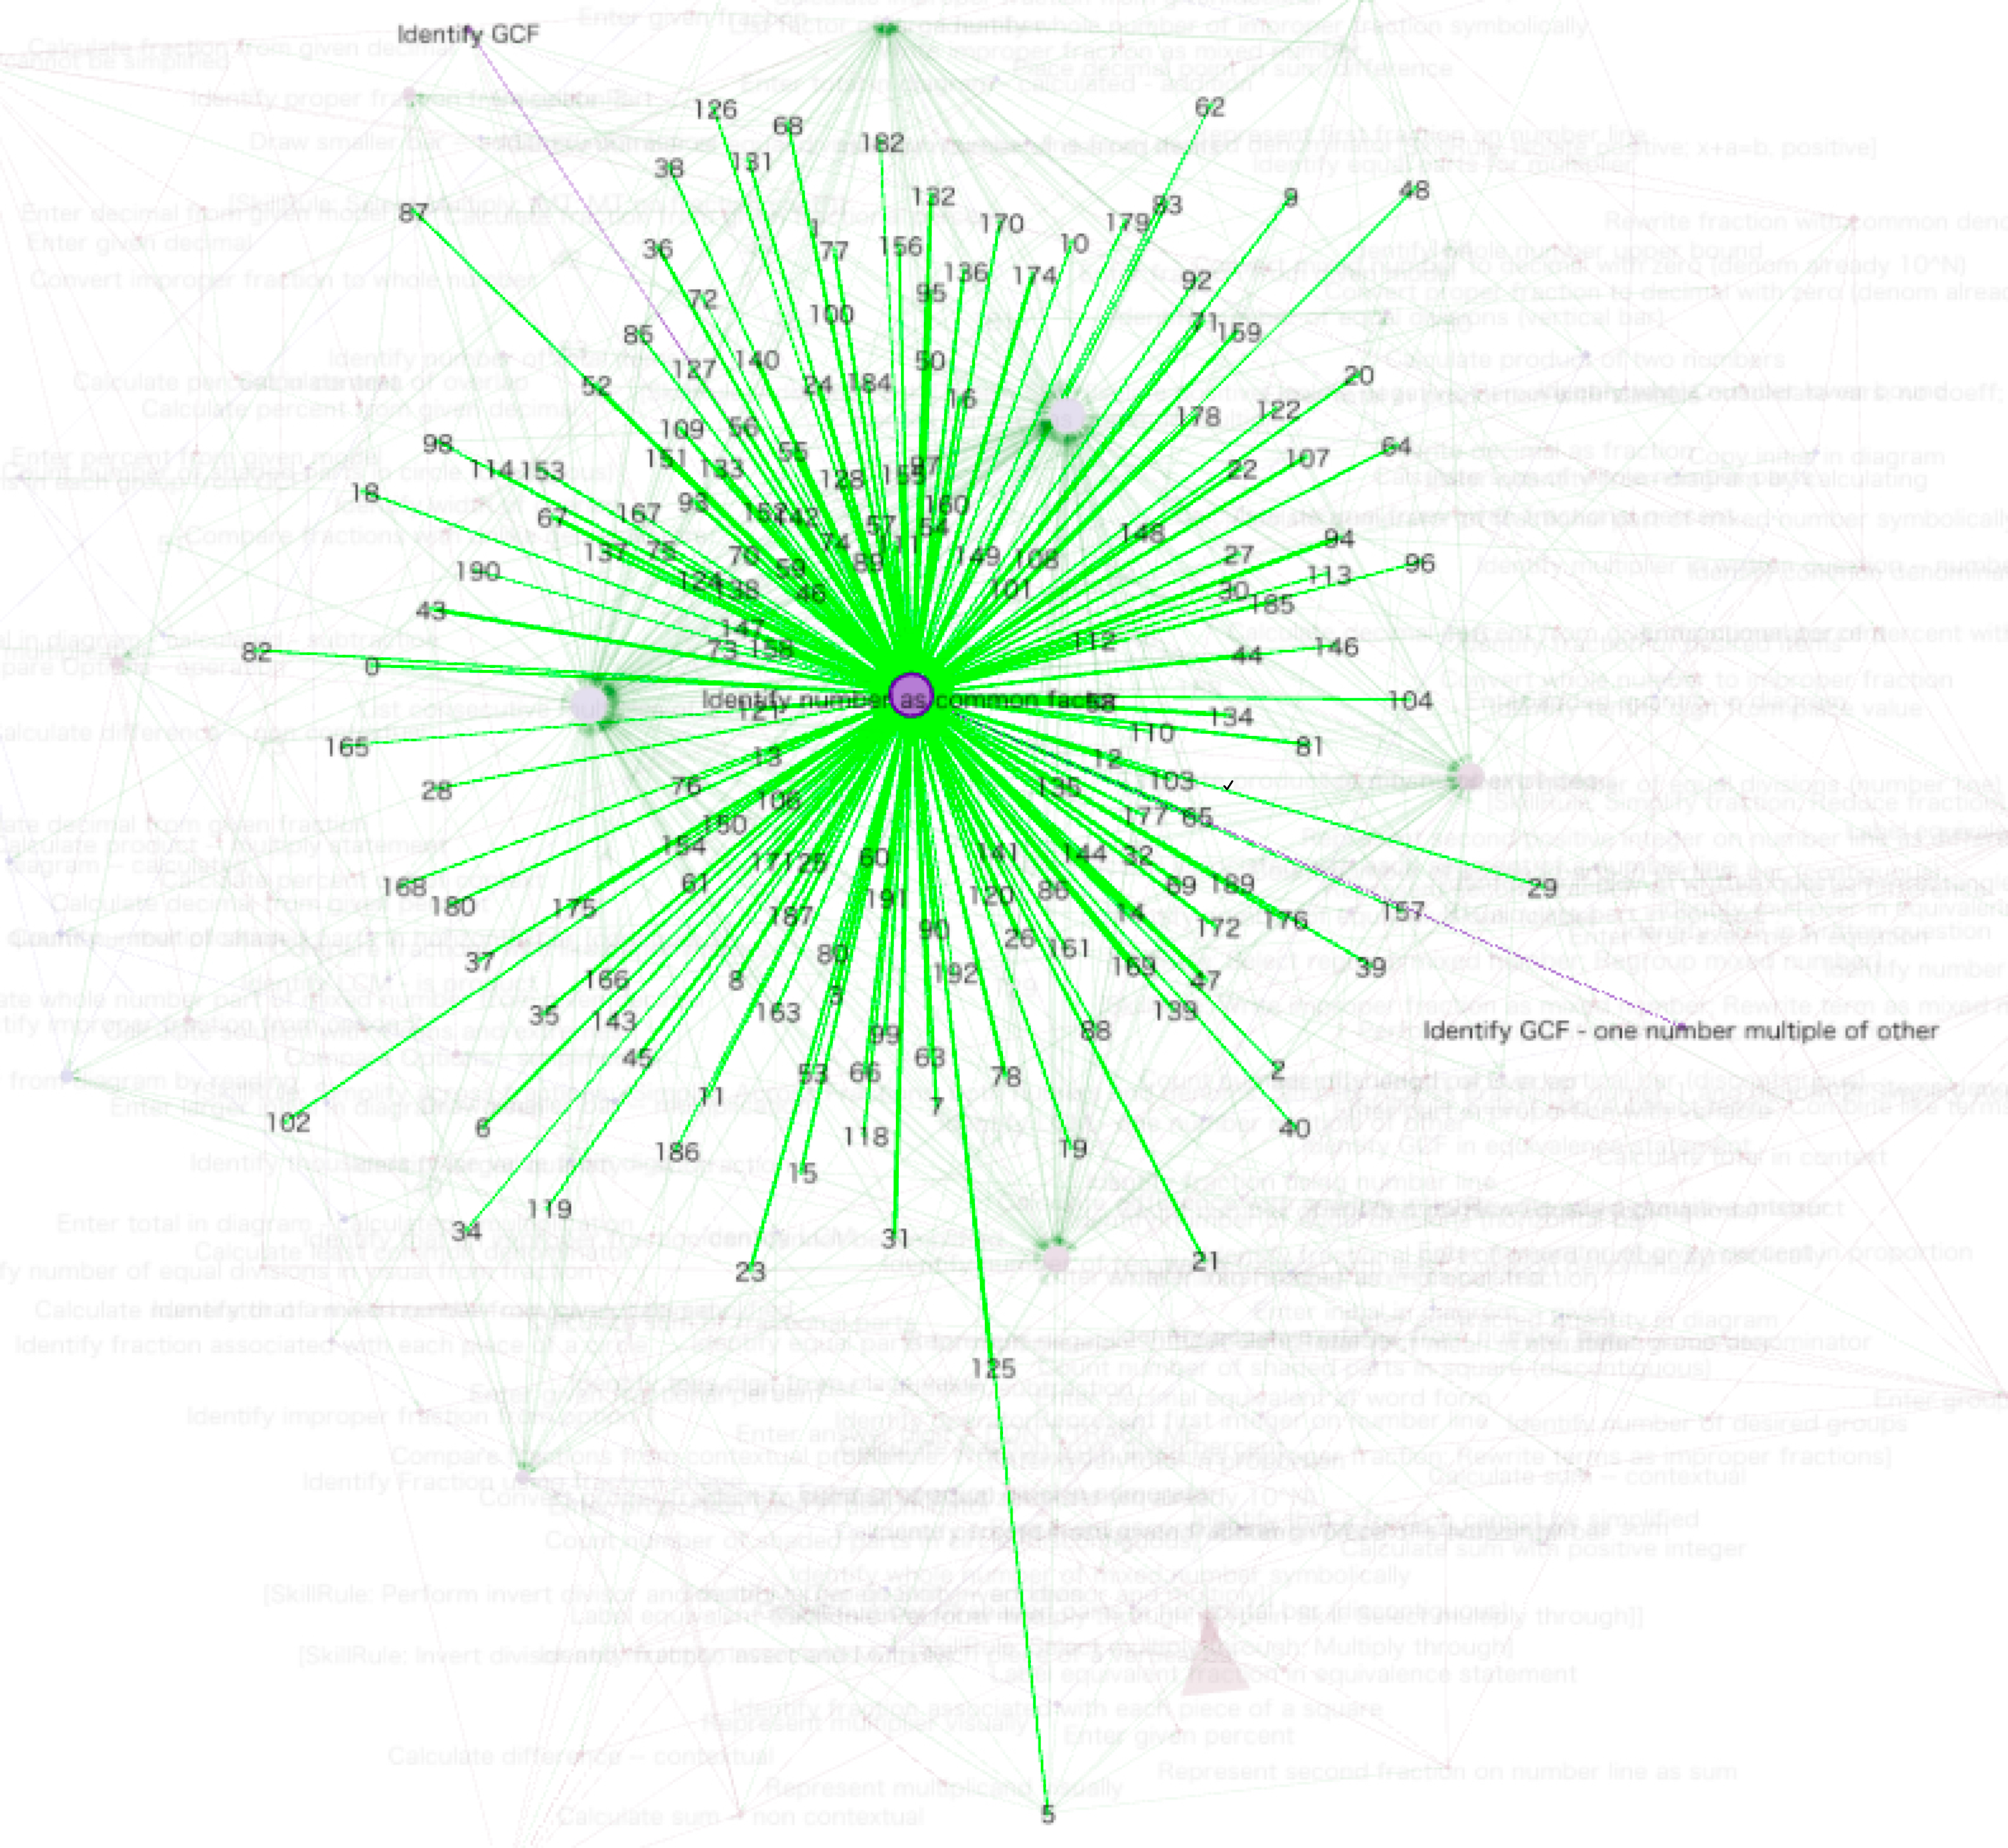
\includegraphics[height=120pt]{./img/kNetworkConcentrate2.pdf}
		\subcaption{「Bridge to Algebra 2006-2007」}
	\endminipage\hfill
}
\end{center}
\caption{多くの抽出タグが紐づく既存タグ}
\label{fig:NetworkConcentrate}
\end{figure}

\begin{figure}[htb]
\begin{center}
%\hspace*{-40pt}\makebox[1.2\textwidth][c]{
\hspace*{-20pt}\makebox[1.1\textwidth][c]{
	\minipage{0.53\textwidth}
		\centering
		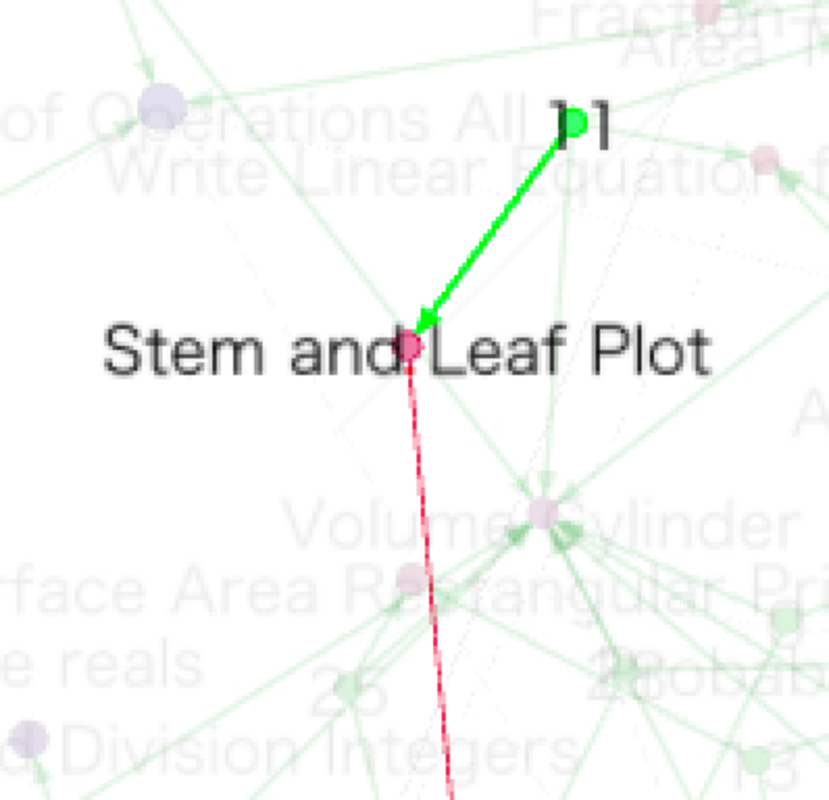
\includegraphics[height=120pt]{./img/aNetworkLittle2.pdf}
		\subcaption{「ASSISTments 2009-2010」}
	\endminipage\hfill
	\minipage{0.53\textwidth}
		\centering
		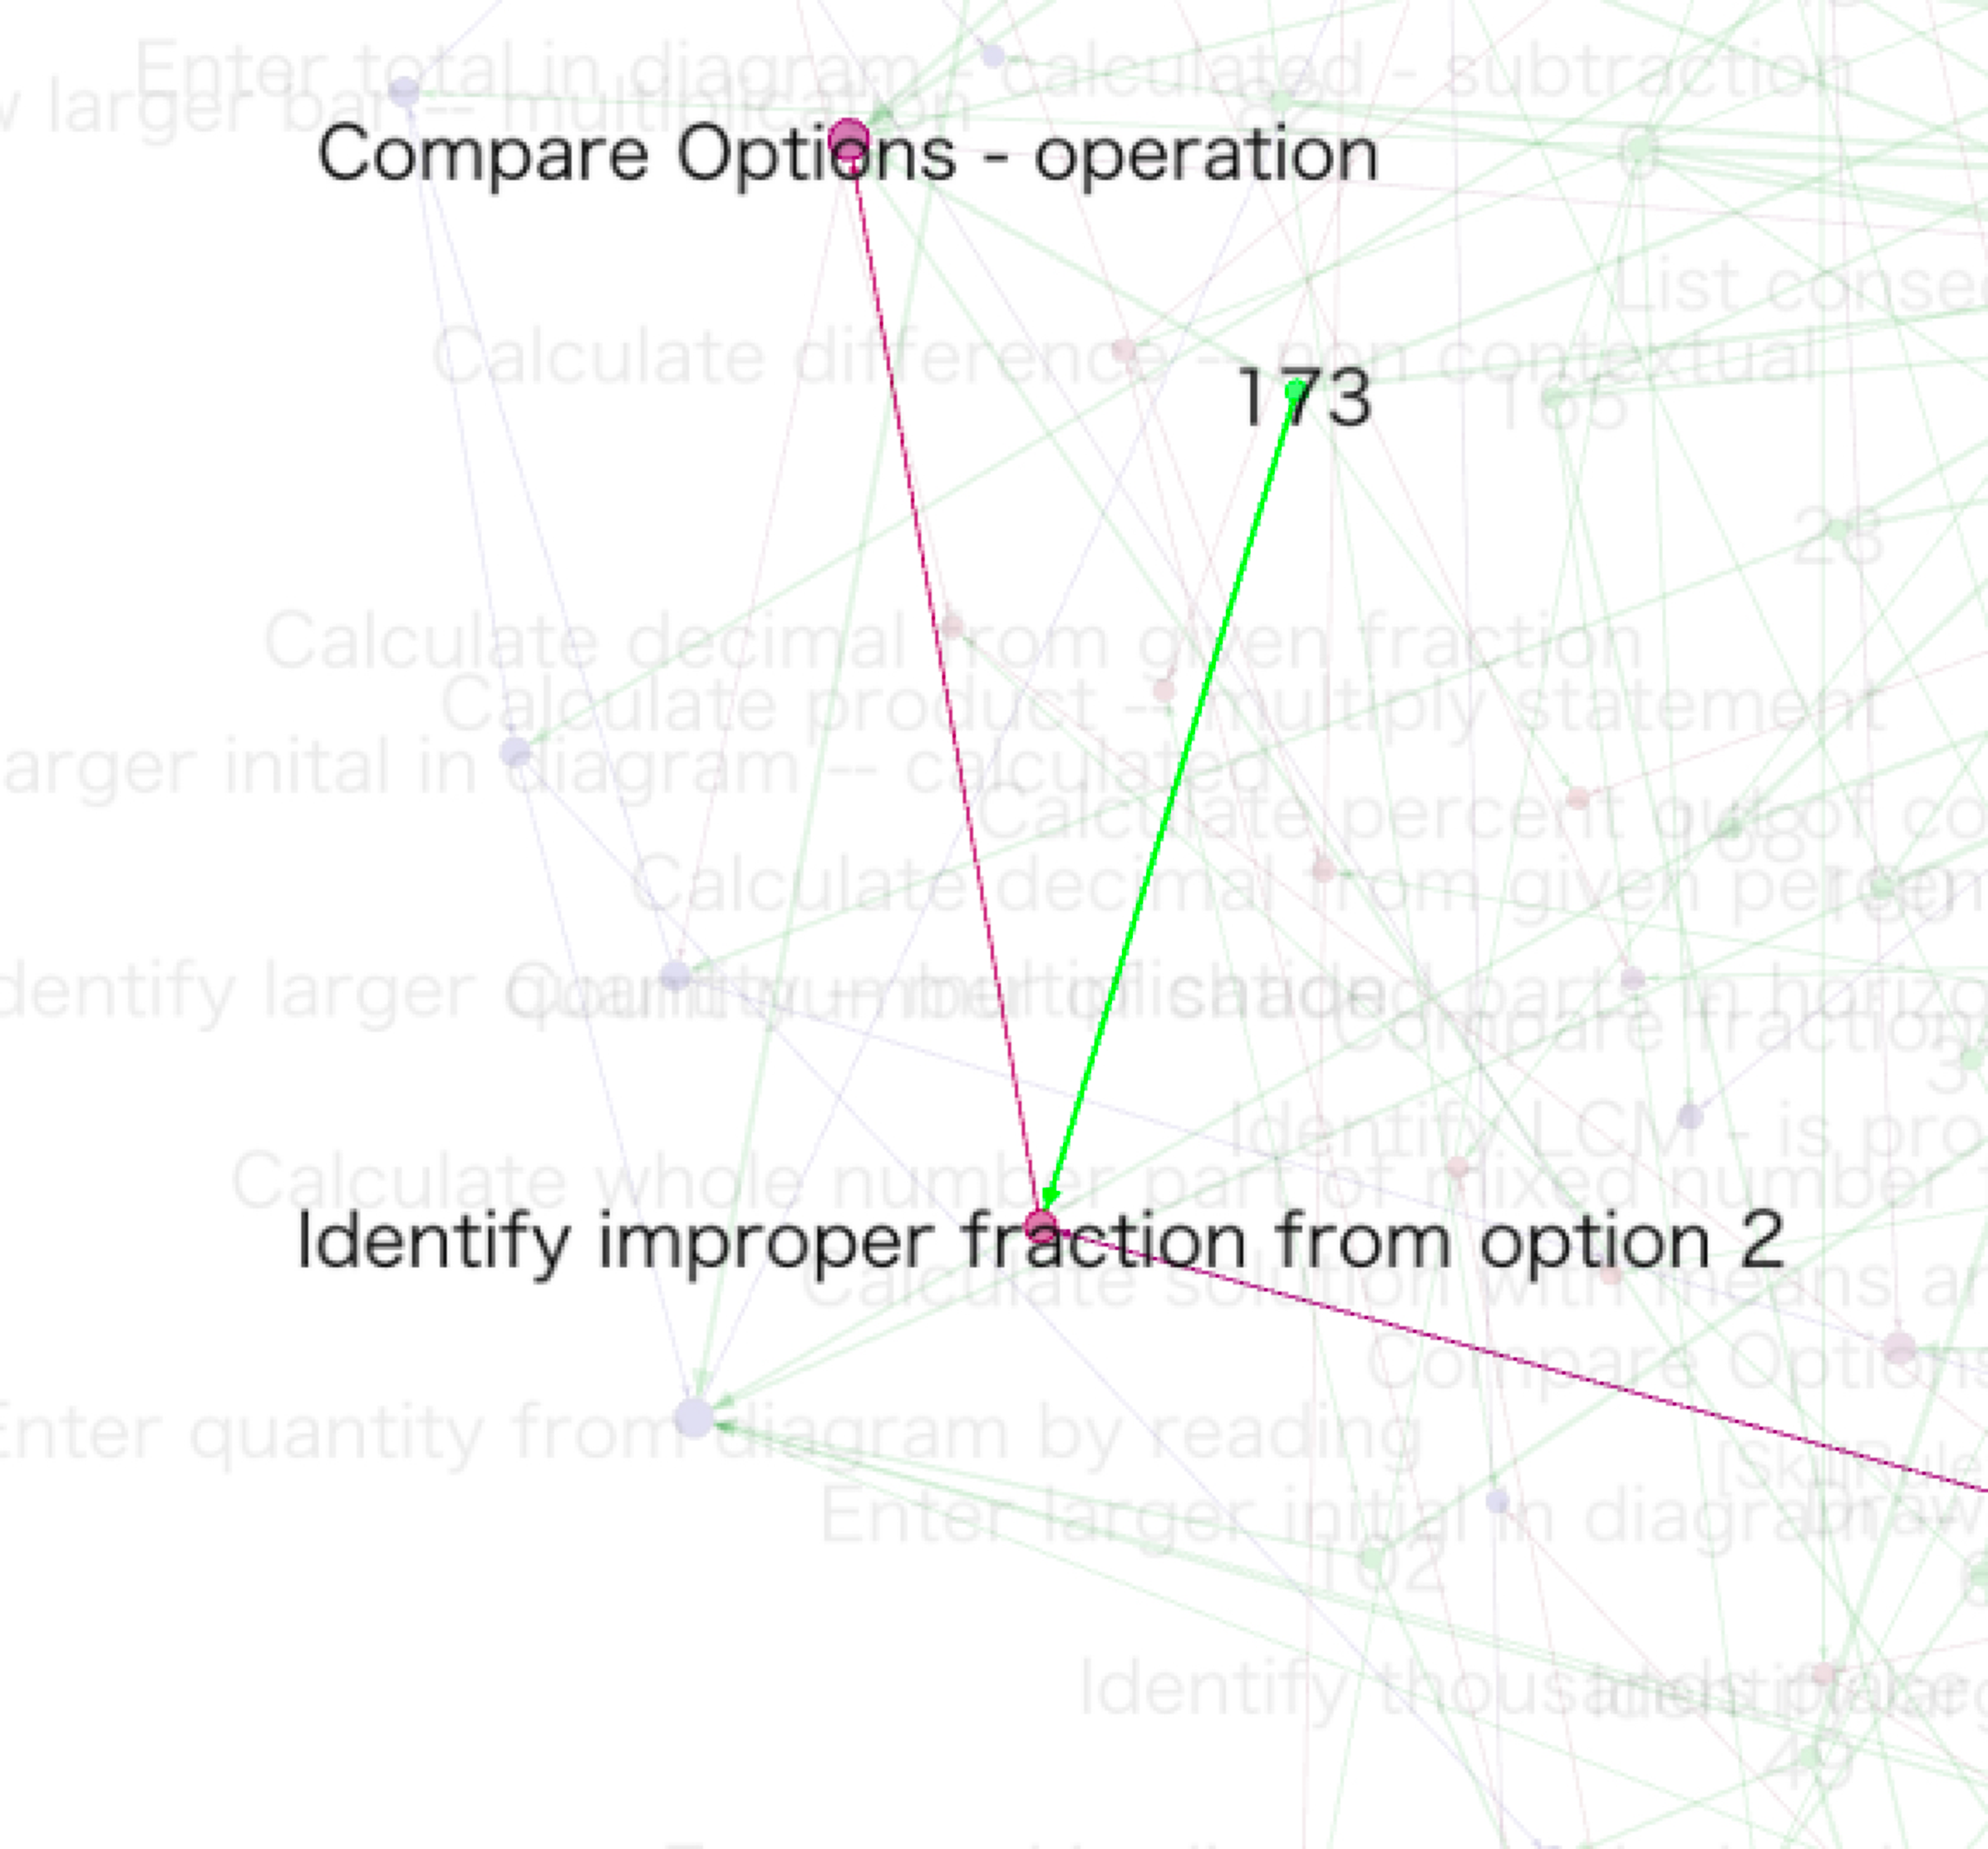
\includegraphics[height=120pt]{./img/kNetworkLittle2.pdf}
		\subcaption{「Bridge to Algebra 2006-2007」}
	\endminipage\hfill
}
\end{center}
\caption{少数の抽出タグのみ紐づく既存タグ}
\label{fig:NetworkLittle}
\end{figure}

次に,抽出タグに注目し,各抽出タグがどのような既存タグに紐付いているかを観察すると,
内容的な関係性の強い複数の既存タグに紐付いている抽出タグが存在する(図\ref{fig:NetworkSimilar})ことがわかる.	
このような既存タグと抽出タグの関係性から,どのような性質のタグが抽出されているといえるかは,第6章で考察する.

\begin{figure}[htb]
\begin{center}
%\hspace*{-40pt}\makebox[1.2\textwidth][c]{
\hspace*{-20pt}\makebox[1.1\textwidth][c]{
	\minipage{0.53\textwidth}
		\centering
		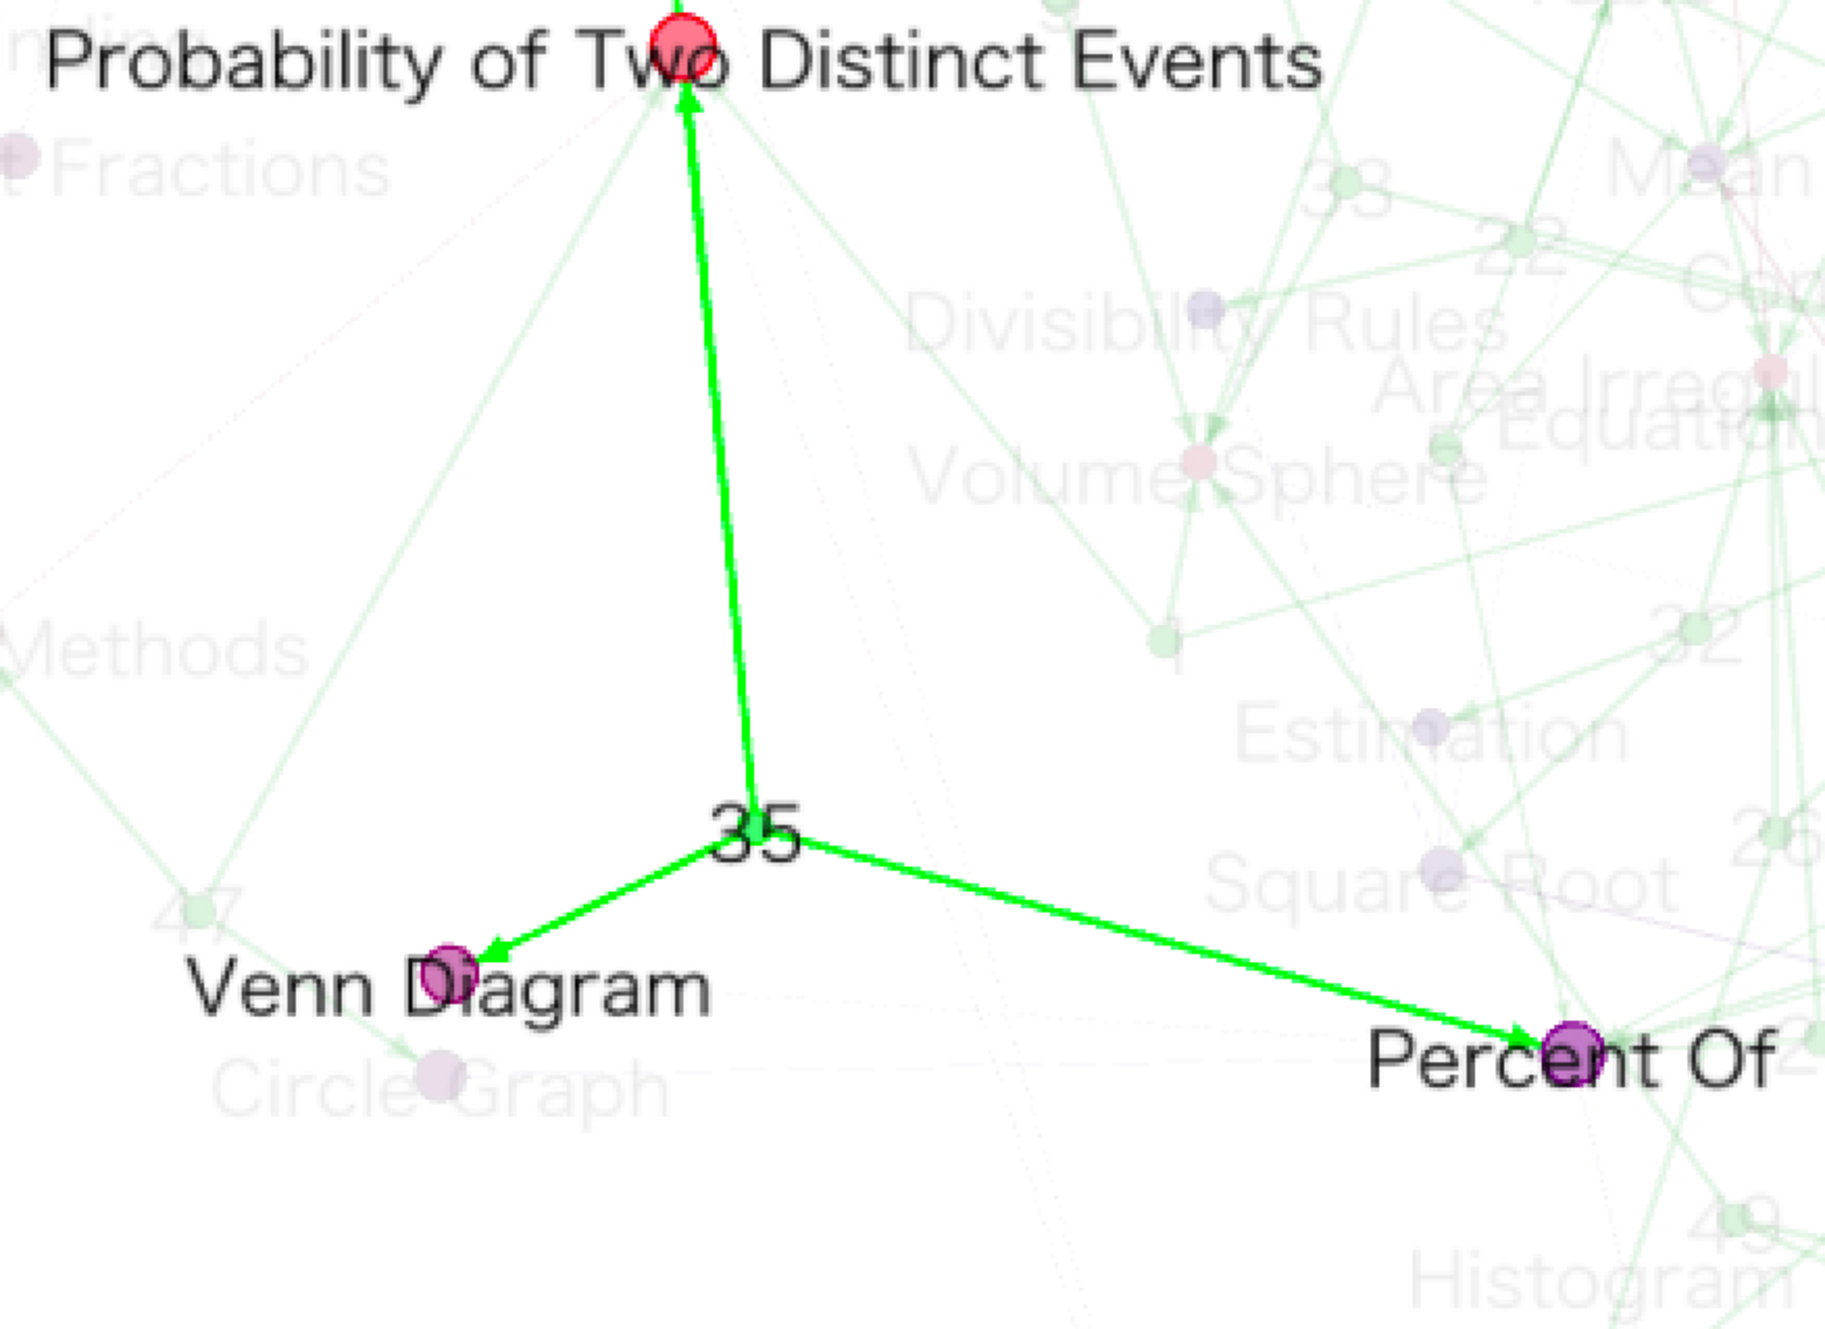
\includegraphics[height=120pt]{./img/aNetworkSimilar2.pdf}
		\subcaption{「ASSISTments 2009-2010」}
	\endminipage\hfill
	\minipage{0.53\textwidth}
		\centering
		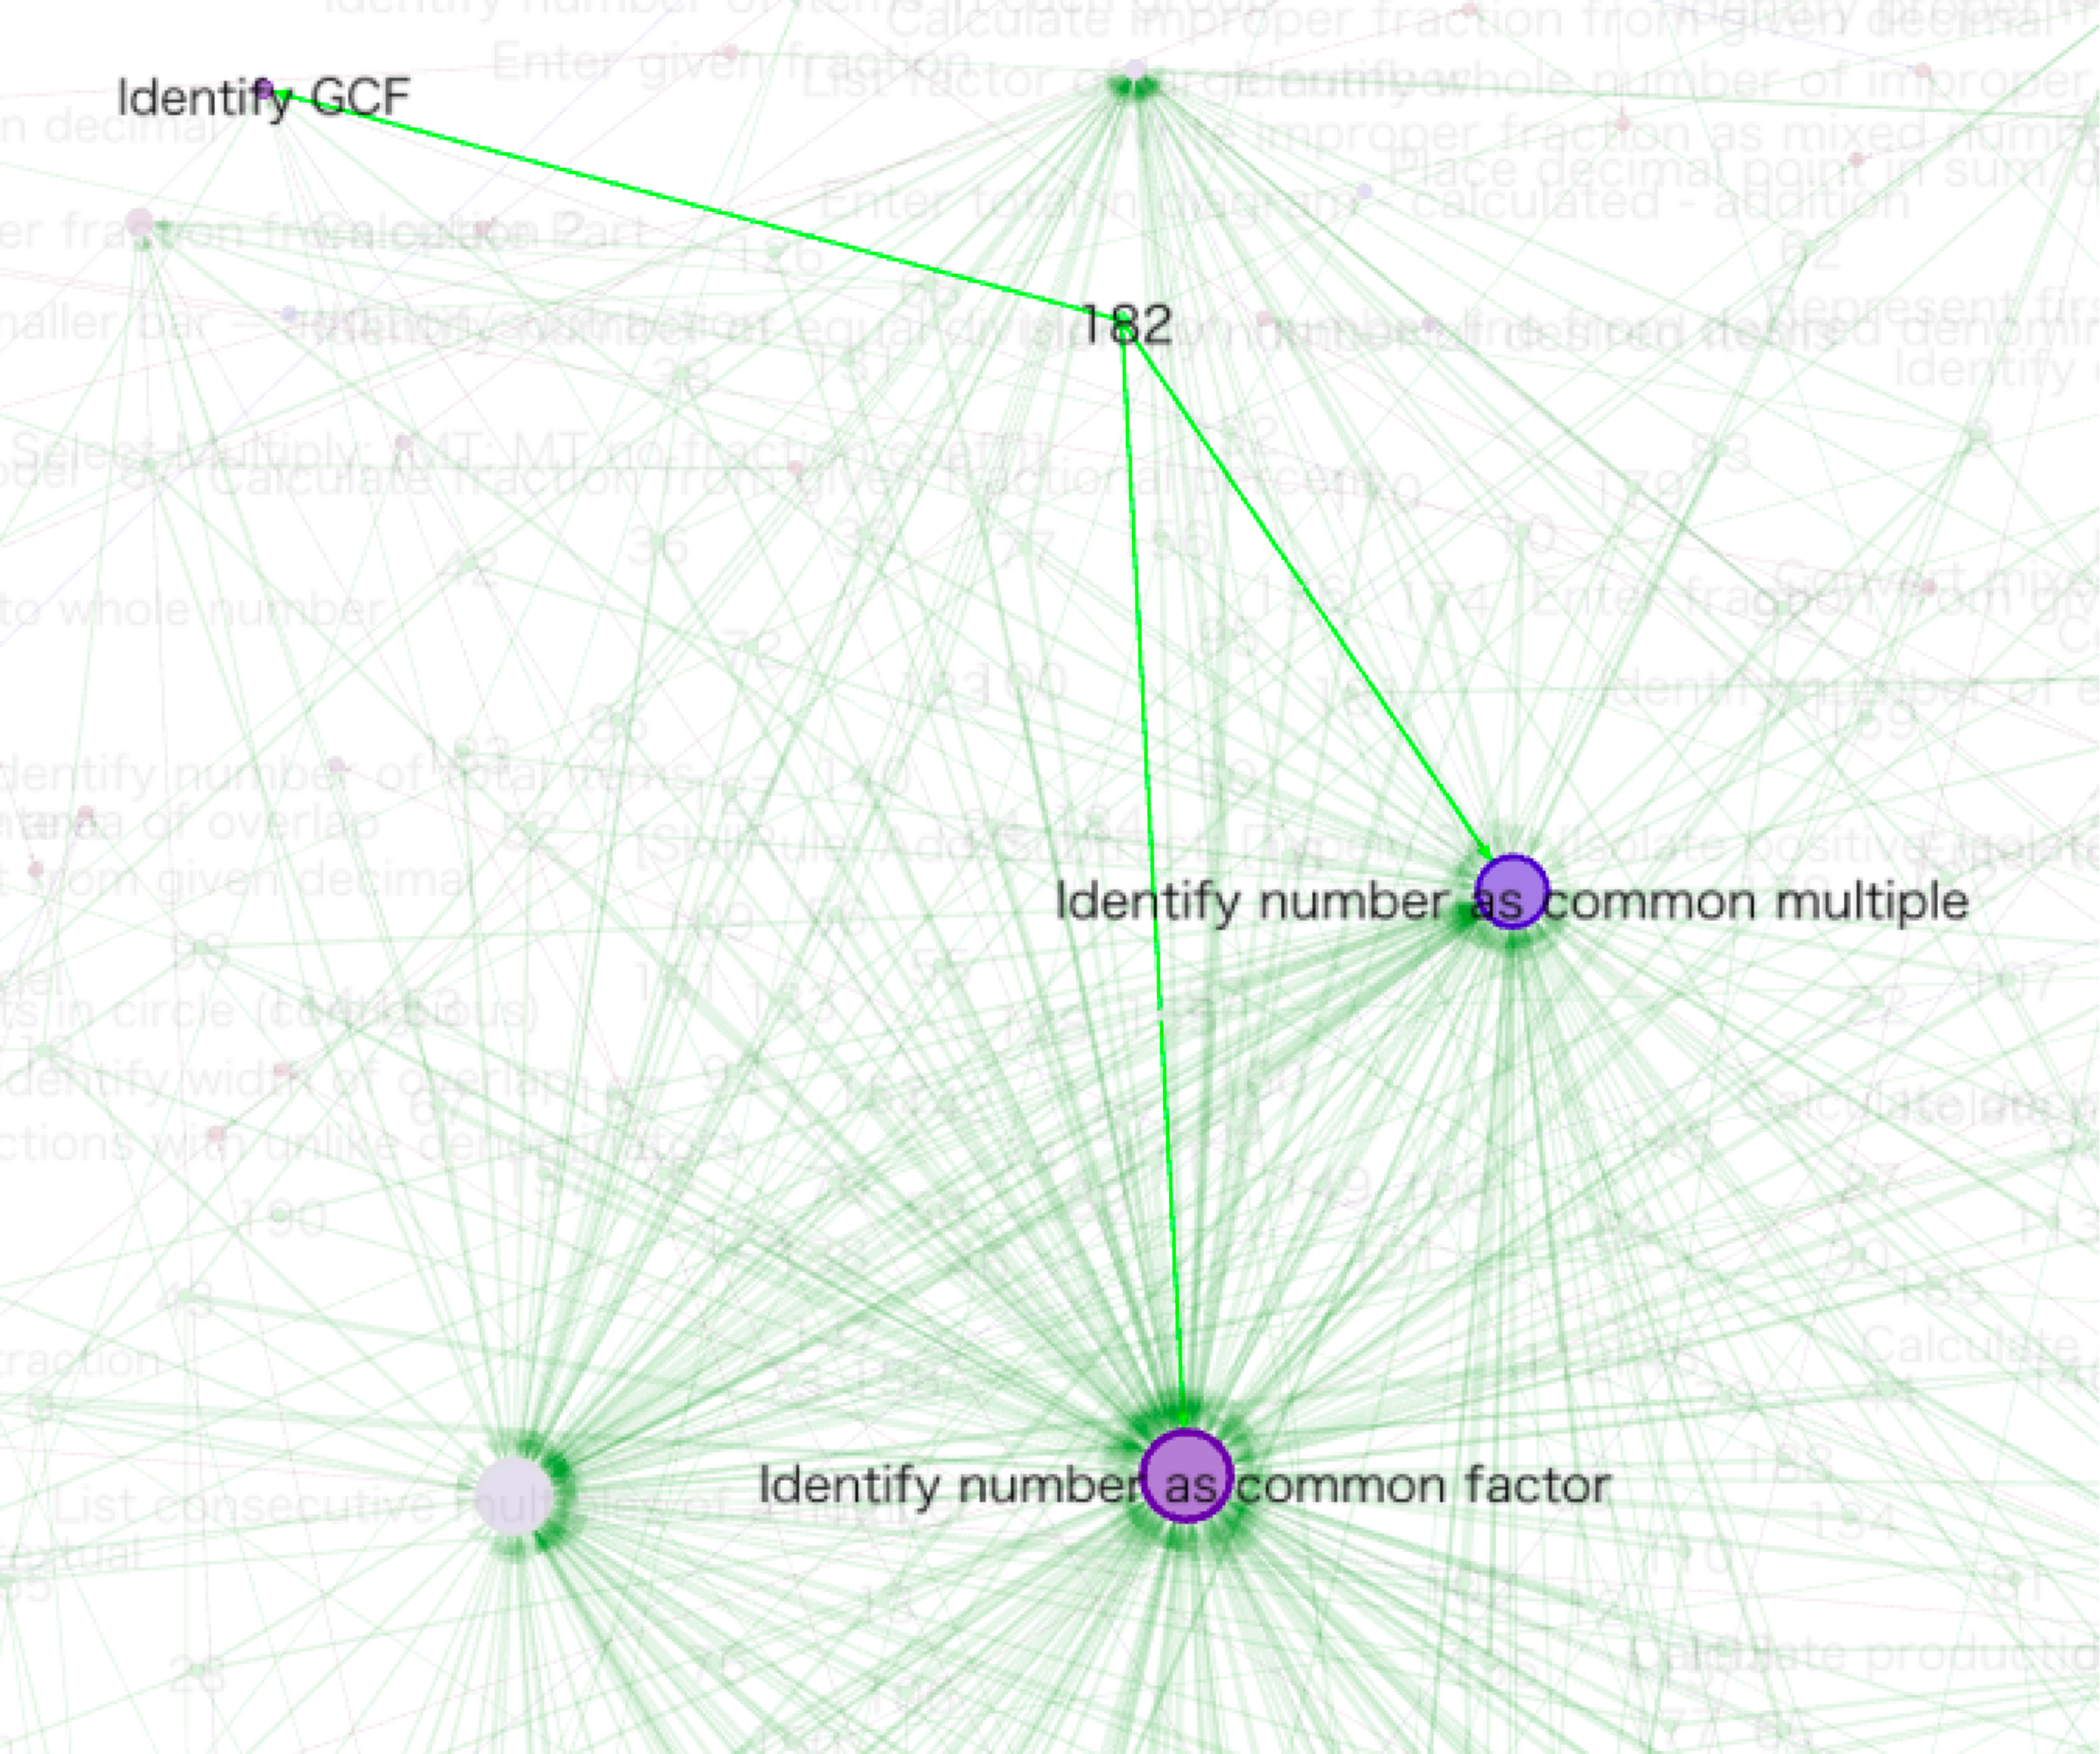
\includegraphics[height=120pt]{./img/kNetworkSimilar2.pdf}
		\subcaption{「Bridge to Algebra 2006-2007」}
	\endminipage\hfill
}
\end{center}
\caption{内容的関係性の強い既存タグに紐づく抽出タグ}
\label{fig:NetworkSimilar}
\end{figure}

